\documentclass[preprint,5p]{elsarticle}



\usepackage{natbib}
\bibliographystyle{abbrvnat}
\setcitestyle{authoryear,open={(},close={)}} \setcitestyle{citesep={;}} \usepackage{graphicx}
\usepackage{footnote}
\makesavenoteenv{tabular}
\makesavenoteenv{table}
\usepackage{multicol}

\usepackage[printwatermark]{xwatermark}
\usepackage{xcolor, colortbl}
\usepackage{tikz}
\newsavebox\mybox
\savebox\mybox{\tikz[color=gray,opacity=0.3]\node{DRAFT};}
\newwatermark*[
  allpages,
  angle=45,
  scale=11,
  xpos=-30,
  ypos=30
]{\usebox\mybox}


\usepackage{url}
\usepackage{amssymb}


\usepackage{dcolumn}\usepackage{bm}\usepackage[switch]{lineno}


\usepackage{caption}
\usepackage{subcaption}
\usepackage{amsmath}


\DeclareCaptionType{equ}[Equation][List of Equations]







\journal{Astronomy And Computing}

\begin{document}\sloppy
\definecolor{Gray}{gray}{0.9}
\begin{frontmatter}



\title{Scalability Model for the LOFAR Direction Independent Pipeline}\author{A.P. Mechev $^a$}
\ead{apmechev@strw.leidenuniv.nl}

\author{T.W. Shimwell $^b$}\author{A. Plaat $^c$}\author{H. Intema $^{ad}$}\author{A.L. Varbanescu $^e$}
\author{H.J.A Rottgering $^a$}

\date{\today} 
\address{$^a$ Leiden Observatory, Niels Bohrweg 2, 2333 CA Leiden, the Netherlands}
\address{$^b$ ASTRON, Oude Hoogeveensedijk 4, 7991 PD , The Netherlands }
\address{$^c$ Leiden Institute of Advanced Computer Science, Niels Bohrweg 1, 2333 CA Leiden, the Netherlands}
\address{$^d$ International Centre for Radio Astronomy Research -- Curtin University, GPO Box U1987, Perth, WA 6845, Australia}
\address{$^e$ University of Amsterdam, Spui 21, 1012 WX Amsterdam, the Netherlands}


\begin{abstract}
LOFAR is a leading aperture synthesis telescope operated by the Netherlands with stations across Europe. The multi-Petabyte, LOFAR Two-meter Sky Survey (LoTSS) will produce more than 3000 14 TB data sets, all of which need to be processed by the LOFAR Direction Independent (DI) pipeline. Understanding the performance of the DI pipeline is important when trying to optimize the throughput for its large projects, such as LoTSS and other deep surveys. Making a model of its completion time will enable us to predict the time taken to process large data sets, optimize our parameter choices, help schedule other LOFAR processing services, and predict processing time for future large radio telescopes. We tested the full LOFAR target calibration pipeline (\texttt{prefactor}) by scaling several parameters, notably number of CPUs, data size and size of calibration sky model. We present these results as a comprehensive model which will be used to predict processing time for a wide range of processing parameters. We also discover that smaller calibration models lead to significantly faster calibration times, while the calibration results do not significantly degrade in quality. Finally, we validate the model and compare predictions with production runs from the past six months, quantifying the performance penalties incurred by processing on a shared cluster. 

\end{abstract}
\begin{keyword}
Radio Astronomy \sep Performance Analysis \sep Performance Modelling \sep High Performance Computing \sep Scalability




\end{keyword}
\end{frontmatter}



\section{\label{sec:intro}Introduction }

Astronomy has entered the big data era with many projects creating Petabytes of data per year. This data is often processed by complex multi-step pipelines consisting of various algorithms. Understanding the scalability of astronomical algorithms theoretically, in a controlled environment, and in production is important to making prediction for future projects and upcoming telescopes. 

The Low Frequency Array (LOFAR) \citep{LOFAR} is a leading European low-frequency radio telescope. The majority of LOFAR's stations are in the Netherlands, however it can use stations across Europe to create ultra-high resolution radio maps.  LOFAR data needs to undergo several computationally intensive processing steps before obtaining a final scientific image. 

To create a broadband image, LOFAR data is first processed by a Direction Independent (DI) Calibration pipeline followed by Direction Dependent (DD) Calibration pipeline \citep[e.g.][]{lofar_prefactor, Wendy_bootes,tassesmirnov, tasse2018faceting}. Direction Independent LOFAR processing can be parallelized on a high throughput cluster \citep{mechev17}, while the Direction Dependent processing is typically performed on a single HPC node. 

The LOFAR Surveys Key Science Project (SKSP) \citep{lotss, LOTSS_DR2} is a long running project with the aim of creating a deep image of the northern sky at low frequencies. The broadest tier of the survey will use more than 3000 8-hour observations to create maps with a noise levels below 100 $\mu$Jy. We have already processed more than 500 of these observations using the \texttt{prefactor} direction independent software \citep{lofar_prefactor, prefactor_zenodo}. 

While the current imaging algorithms can process data averaged by a factor of 64 in frequency and time, it is important to understand how LOFAR processing scales with processing parameters, such as averaging parameters. With increasing LOFAR observation rates, data sizes and scientific requirements, users need to be able to predict the time and computational resources required to process their data.  We study the scalability of LOFAR processing, by setting up processing of a sample SKSP data set on an isolated node on the \texttt{GINA} cluster at SURFsara, part of the Dutch national e-infrastructure \citep{dutch_einfra}. We tested the software performance as a function of several parameters, including averaging parameters, number of CPUs and calibration model size. Additionally, we tested the performance of the underlying infrastructure, i.e. queuing  and download time, for the same parameters. Finally, we compared the isolated tests with our production runs of the \texttt{prefactor} pipeline to measure the overhead incurred by running on a shared system. 

We discover that the intensive LOFAR processing steps scale linearly with data size, and calibration model size. Additionally, we find that the time taken by these steps is inversely proportional to the number of CPUs used. We discover that the time to download and extract data on the \texttt{GINA} cluster is linear with size up to 32GB, however becomes slower beyond this data size. We also find that the queuing time on the \texttt{GINA} cluster grows exponentially for jobs requesting more than 8 CPUs. We validate these isolated tests with production runs of LOFAR data from the past six months.  Finally we combine all these tests into a single model and show its prediction power by testing the processing time for different combinations of parameters. The major contributions of this work can be summarized as:

\begin{itemize}
    \item A model of processing time for the  LOFAR Direction Independent Calibration Pipeline.
    \item A model of queueing time and file transfer time which is used by current or future jobs processed on the \texttt{GINA} cluster.
    \item Quantification of overheads incurred when processing in production. 
\end{itemize}

We introduce LOFAR processing and other related work in Section \ref{sec:related} and describe our software setup and data processing methods in Section \ref{sec:methods}. We present our results and performance model in Section \ref{sec:results} and discussions and conclusions in Section \ref{sec:discussions}. 


\section{Related Work}\label{sec:related}
In previous work, we have parallelized the Direction Independent LOFAR pipeline on a High Throughput infrastructure \citep{mechev17}. While this parallelization has helped accelerate data processing for the SKSP project, creating a performance model of our software is required if we are to predict the resources taken by future jobs. This model will be particularly useful in understanding how processing parameters will affect run time.  

Performance modelling on a distributed system is an important field of study related to grid computing. A good model of the performance of tasks in a distributed workflows can help more efficiently schedule these jobs on a grid environment \citep{grid_perform_model}. The performance modeling systems require knowledge of the source code and an analytical model of the slowest parts of the code \citep{semi_analytical_model}. Many systems exist to model the performance of distributed jobs \citep{barnes2008regression, semi_analytical_model,performance_prediction,Witt2018PredictivePM}, with some employing Black Box testing \citep{cross_platform_black_box, mapreduce_analysis} or tests on scientific benchmark cases \citep{synthetic_memory_prediction}. Such performance analysis does not require intimate knowledge of the software and can be applied on data obtained from processing on a grid infrastructure.

Empirical modelling is useful in finding performance bugs in parallel code \citep{scalability_bugs} and modelling the performance of big data architectures \citep{mean_field_modeling}. The insights from these models are used to optimize the architecture of the software system or determine bottlenecks in processing. Here, we use empirical modelling to determine how the LOFAR \texttt{prefactor} performance scales with different parameters. 


\section{Processing Setup }\label{sec:methods}
\interfootnotelinepenalty=10000
Using the LOFAR software install described in \cite{mechev17}, we processed a typical LOFAR SKSP observation\footnote{LOFAR Observation ID L658492, co-ordinates [17h42m21.785, +037d41m46.805] observed by the LOFAR High Band Array for 8 hours between 2018-06-20 and 2018-06-21.} averaged in time and frequency at different rates. Changing these averaging parameters will change the final data size (with the data sizes studied shown in Table \ref{table:averaging}). We test the processing time for different averaging parameters by running 15 runs per parameter step. 

The processing was done on a dedicated node of the SURFsara \texttt{GINA} cluster, f18-01. The node is a typical processing node used by our LOFAR Surveys processing, however it is dedicated for the tests in order to ensure there is no contamination by other processes. The node is described in Section \ref{sec:hardware}. 
     


We processed the sample data set with the LOFAR \texttt{prefactor} pipeline. The \texttt{prefactor} version used was the same as we use for the LOFAR SKSP broadband surveys \citep{prefactor_zenodo}. This software consists of several steps executed in sequence, shown graphically in Figure \ref{fig:prefactor_steps}. The important \texttt{prefactor} steps are as follows. The Predict\_ateam and ateamcliptar steps predict the contamination by bright off-axis sources and remove these effects respectively. The dpppconcat step is responsible for concatenating 10 subbands into a single file which is in turn calibrated. The step gsmcal\_solve is responsible for calibration of the data against a model of the radio sky. The solutions produced by gsmcal\_solve is used by gsmcal\_apply and applied to the scientific observation.

\begin{figure}
    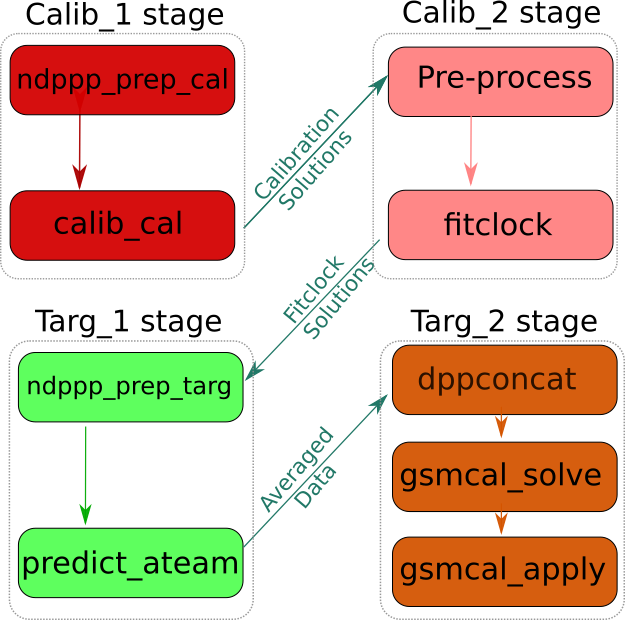
\includegraphics[width=0.95\linewidth]{figures/4_stages_steps1.png}
      \caption{The major steps of the \texttt{prefactor} DI pipeline. }
	\label{fig:prefactor_steps}
\end{figure}

\subsection{Processing Metrics}
The goal for our scalability model is to understand the effect of several parameters on the job completion time of LOFAR software. We do this by testing the processing time for various values of data size, number of CPUs used and sky model size. 

The data used by the LOFAR surveys is archived at a time resolution of 1 second intervals and frequency resolution of 16 channels per Subband (equivalent to 12kHz channel width). While some of the processing steps such as flagging of Radio Frequency Interference and removal of bright off-axis sources produce better results when performed on the high-resolution data. Later steps can be performed on averaged data with little impact on the final product quality. To speed up processing, the raw data is averaged in time and frequency, decreasing the input data size to later tasks. The main aims of the LOFAR surveys project can be accomplished if the final data products from the prefactor pipeline are averaged to a resolution of 8 seconds per sample and 2 channels per subband. These averaging parameters correspond to a reduction in size by a factor of 64. In Section \ref{sec:results_size}, we measure the performance of the \texttt{prefactor} pipeline for data sizes between the raw data of 64GB/Subband and the averaged data of 1GB/Subband. The tested data sizes and parameters are shown in table \ref{table:averaging}. 


\begin{table}[!ht]
\centering
\begin{tabular}{||c| c | c | c||} 
 \hline
 Data set & \multicolumn{1}{|p{2cm}|}{\centering Time averaging \\ parameter (sec)} &  \multicolumn{1}{|p{2cm}|}{\centering Channels per Subband} & Size (Gb) \\ [0.5ex]
 \hline
 \rowcolor{Gray}
  \hline
 1GB & 8   & 2   &  1.235   \\ 
  \hline
 2GB & 4   & 2   &  2.459   \\ 
 4GB & 2   & 2   &  4.906   \\ 
 8GB & 1   & 2   &  9.802   \\ 
 16GB & 1   & 4   &  18.00  \\ 
 32GB & 1   & 8   &  36.72  \\ 
 64GB & 1   & 16   &  66.88  \\[1ex] 
 \hline
\end{tabular}
\caption{Averaging parameters and final data sizes tested for the sample LOFAR SKSP observation. The raw data is 64 GB per Subband. The LOFAR SKSP data processing uses averaging parameters of 8 seconds and 2 channels per Subband. This reduces the raw data by a factor of 64. We highlight the data size used in the LOFAR SKSP survey.   }
\label{table:averaging}
\end{table}

The slowest step of the \texttt{prefactor} pipeline is the gsmcal\_solve step, which performs the gain calibration against a model of the radio sky. This step operates on a concatenated data set that consists of 10 subbands. We obtain the calibration model through the TGSS sky model creator\footnote{Accessible at \href{http://tgssadr.strw.leidenuniv.nl/doku.php}{the TGSS ADR portal}.}. By default this service creates a text file describing the sky-model from the TGSS survey \citep{tgssadr}. By default, it sets a threshold of sources brighter than 0.3 Jy. 
Lowering this threshold creates longer sky-model files with more faint sources, while increasing it will return only the few brightest sources. Since sky model calibration requires converting the sky-model into modelled visibilities \citep[e.g.][]{dppp, radio_visibility_sage,app_synth}, a longer sky model will increase the time taken to gain calibrate a data set. We created 7 sky models with a flux cutoff ranging between 0.05 Jy and 1.5 Jy. The number of sources in the resulting models are listed in Table \ref{table:skymodels}. 
For production\footnote{The query used to obtain model 3 is at the following link \url{http://bit.ly/tgss_model}}, we used the minimum sensitivity parameters for model 3.


It is important to note that the complexity and accuracy of the sky model depend on the direction of observation and the conditions in which the observation was performed. As such, our test is only a heuristic for predicting the run-time based on the calibration model length. Additionally, it is notable that the number of sources is an exponentially dependent on the minimum sky model sensitivity (seen in Figure \ref{fig:skymodel_size}, more in \citealt{tgssadr,Wendy_bootes}). According to this relationship, even a modest decrease in sensitivity cutoff can significantly decrease the size of the model.

\begin{table}[!ht]
\centering
\begin{tabular}{||c| c | c||} 
 \hline
 Sky model \# & min sensitivity & \# sources  \\ [0.5ex] 
 \hline
 model 1 & 0.05 Jy & 809    \\ 
 model 2 & 0.1 Jy & 503   \\
 \rowcolor{Gray}
  \hline
 model 3 & 0.3 Jy & 180   \\
  \hline
 model 4 & 0.5 Jy & 96  \\
 model 5 & 0.8 Jy & 49   \\ 
 model 6 & 1.0 Jy & 34   \\
 model 7 & 1.5 Jy & 16   \\[1ex] 
 \hline
\end{tabular}
\caption{List of test sky models. Model 3 is created with the parameters used in our production processing of LOFAR data. All models include objects within 5 degrees from the centre of the pointing.  }
\label{table:skymodels}
\end{table}


\begin{figure}
    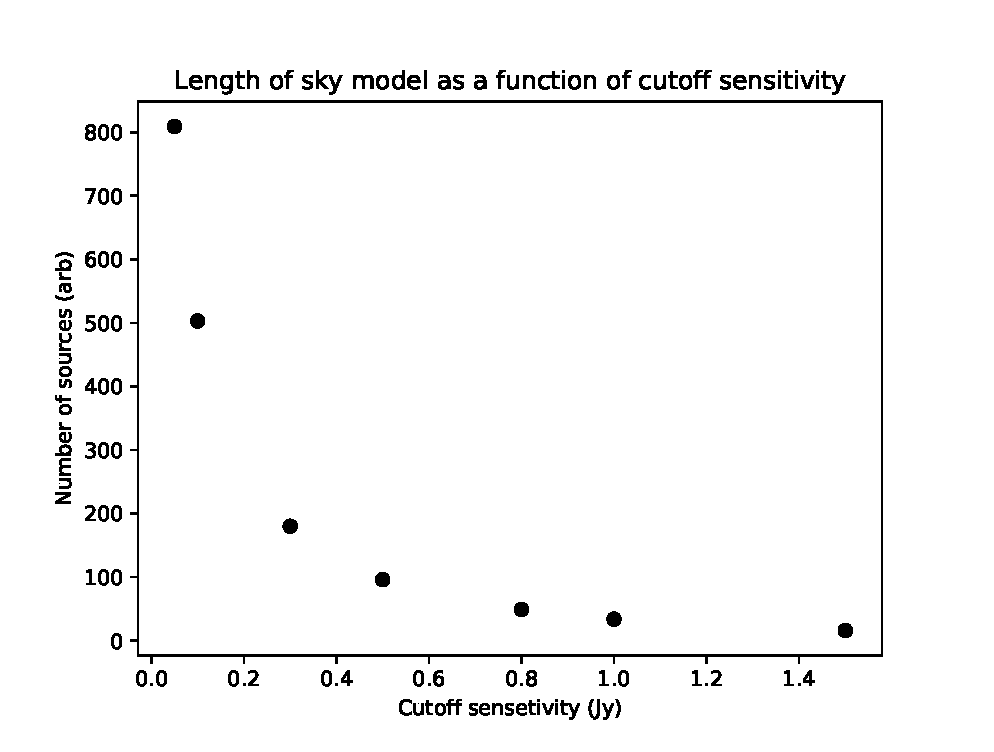
\includegraphics[width=0.95\linewidth]{figures/skymodel_size_vs_Jy.eps}
      \caption{The size of the sky model (measured in number of sources) increases exponentially as we decrease the flux cutoff of the model (i.e. increase the sensitivity).}
	\label{fig:skymodel_size}
\end{figure}


Finally, the number of CPUs used by each step is a parameter that can be optimized for the entire pipeline. While increasing the number of CPUs can make some steps run faster, requesting jobs that reserve a large number of CPUs will take longer to launch on shared infrastructure. In order to understand the interplay between these effects, we study the queuing time and processing time as a function of number of CPUs. For the parameter steps we choose to test 1, 2, 3, 4, 8 and 16 CPUs. 

\subsection{Infrastructure Performance}


Since our jobs are launched on a cluster supporting several different use cases, the requested resources are allocated by a job queue, in our case implemented by the glite workload management system \citep{glite-wms}. As queuing jobs can take a significant amount of time, we test the queuing time as a function of number of requested CPUs. In order to do that, we create test jobs that log the launch time and submit them, requesting 1, 2, 3, 4, 8 and 16 CPUs. We run 10 to 15 tests for each parameter step to ensure that we capture system variability at different times of day during the week and the weekend. 

Besides queuing, time is also spent during downloading and unpacking data, as well as packing and uploading the results. Despite using no compression to pack the data, untarring and tarring large files still takes time depending on the system workload. We measure the time taken to transfer and unpack data of different sizes. The data sizes we chose were 0.5GB, 1GB, 2GB, 4GB, 8GB, 16GB, 32GB and 64GB. As our largest data sets are 64GB and our smallest results are $\sim$0.2GB, these values span a realistic range expected for LOFAR data processing. We test this by uploading mock data to the dCache storage pool at SURFsara and launching a small 1 CPU job which downloads and untars the data, logging the start time of each step. We present the results of this test in the next section. 


\subsubsection{Software Versions}\label{sec:software_versions}
For the current test, we use the LOFAR software stack, version 2.20.2\citep{cookbook}. This software was compiled on a virtual machine and distributed using the CERN CVMFS virtually mounted file system \citep{cvmfs2008}. We use this software version and distribution method as it is the same software version and distribution used to process the data for the LOTSS Data Release 1. 

\subsection{Test Hardware}\label{sec:hardware}

The LOFAR software was tested on a reserved node on the SURFsara \texttt{GINA} cluster. The node, f18-01 has 348 GB of RAM, 3TB of scratch space \footnote{More detailed specifications are at \href{http://docs.surfsaralabs.nl/projects/grid/en/latest/Pages/Service/system_specifications/gina_specs.html}{the \texttt{GINA} specification page linked here}}. The CPU is an Intel Xeon(R) Gold 6148 CPU with 40 cores clocked at 2.40GHz.  As this hardware node was reserved, there was no other scientific processing aside from our tests, meaning there was no resource contention aside for that inherent in the LOFAR software. In the results section, we compare these isolated runs with processing results over the past two years.  
\section{Results}\label{sec:results}

Using a test data set, we tested the LOFAR \texttt{prefactor} target pipeline on the SURFsara \texttt{GINA} cluster. First we will present the tests done in an isolated environment and then compare them to the run time in production on a shared infrastructure. We will integrate all the results in a complete model which can be used to predict processing time for a variety of parameters. Finally, we will make some predictions on the run time of our processing based on the model and validate these predictions. 

Since we are  processing a sample data set in the context of the LOFAR Surveys project, we will compare these tests with the production runs of our pipeline. In production, the parameters chosen are a data size of 1GB, a sky model length of 180 sources and 8 CPUs for the gsmcal\_solve step. 
 

\subsection{Isolated Environment tests}
We first tested the LOFAR software in isolation in order to determine the scalability of processing time in terms of data size. We run the entire \texttt{prefactor} target pipeline which which removes Direction Independent Calibration errors from a LOFAR science target. In the following sections, we present the models obtained from these tests.  

\subsubsection{Input Data Size}\label{sec:results_size}
LOFAR data can be averaged to different sizes based on the scientific requirements. Smaller data sets are processed faster, so it is important to understand the effect of data size on processing time. We show the processing time for our test data set, averaged to different sizes for several \texttt{prefactor} steps in Figures \ref{fig:predict_ateam}, \ref{fig:ateamcliptar}, \ref{fig:dpppconcat_size}, \ref{fig:gsmcalsolve_size}, \ref{fig:gsmcalapply_size}. The figures also plot linear fits for consecutive pairs of parameter steps, in gray dashed lines, used to help guide the selection of parametric model. 

All of the steps show linear behavior with respect to input data size, while the gsmcal\_solve step is best fit by two linear relationships, for data smaller and larger than 16 GB. The linear fit to the run times are shown in Equations \ref{eq:predictateam}-\ref{eq:gsmcalapply}. The equations show the processing time as a function of the data size ($\mathcal{S}$), with the slope in the units of seconds/byte. The fits are also shown in Figures \ref{fig:predict_ateam} to \ref{fig:gsmcalapply_size} as a black dashed line.

\begin{equ*}
\begin{subequations}
\begin{align}
        T_{predict\_ateam}=5.19\times10^{-8}\mathcal{S}+4.20\times10^1 \label{eq:predictateam} \\
        T_{ateamcliptar}=4.57\times10^{-9}\mathcal{S}-8.42\times10^0 \label{eq:ateamcliptar} \\
        T_{dpppconcat}=3.51\times10^{-8}\mathcal{S}+4.20\times10^1 \label{eq:dpppconcat} \\
        T_{gsmcal\_solve}=\begin{cases}
                          7.38\times10^{-7}\mathcal{S}-8.20\times10^1 &|\mathcal{S}<=1.6\times10^{10}\\
                          1.04\times10^{-6}\mathcal{S}-4.04\times10^3 & |\mathcal{S}>1.6\times10^{10}
    \end{cases} \label{eq:gsmcalsolve} \\
        T_{gsmcal\_apply}=2.07\times10^{-8}\mathcal{S}-1.38\times10^1 \label{eq:gsmcalapply}    
\end{align}
\label{eq:runtime_size_models}
\end{subequations}
\caption{Equations describing the processing time of five \texttt{prefactor} steps as a function of the input data size ($\mathcal{S}$) in bytes.}
\end{equ*}

\begin{figure}
    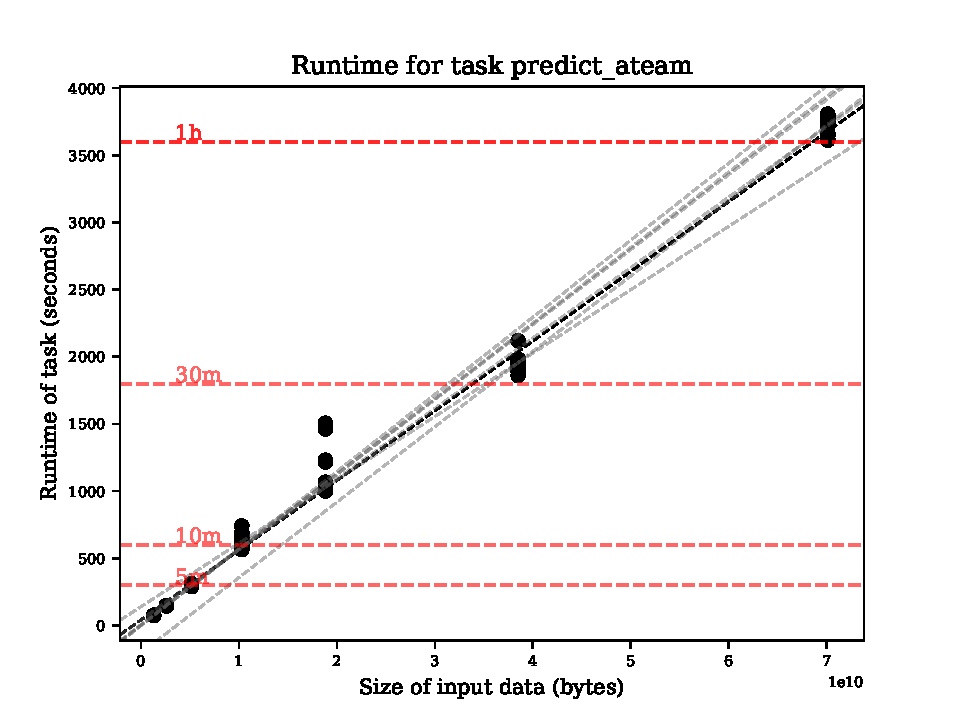
\includegraphics[width=0.95\linewidth]{figures/predict_ateam_size.pdf}
      \caption{Tests of the predict\_ateam step for input data size ranging from 1GB to 64 GB. This step calculates the contamination from bright off-axis sources. Dashed lines are shown connecting each pair of points, to highlight the trend. We can see that the data fits a linear model. We show the model in Equation \ref{eq:predictateam} in black. }
	\label{fig:predict_ateam}
\end{figure}


\begin{figure}
    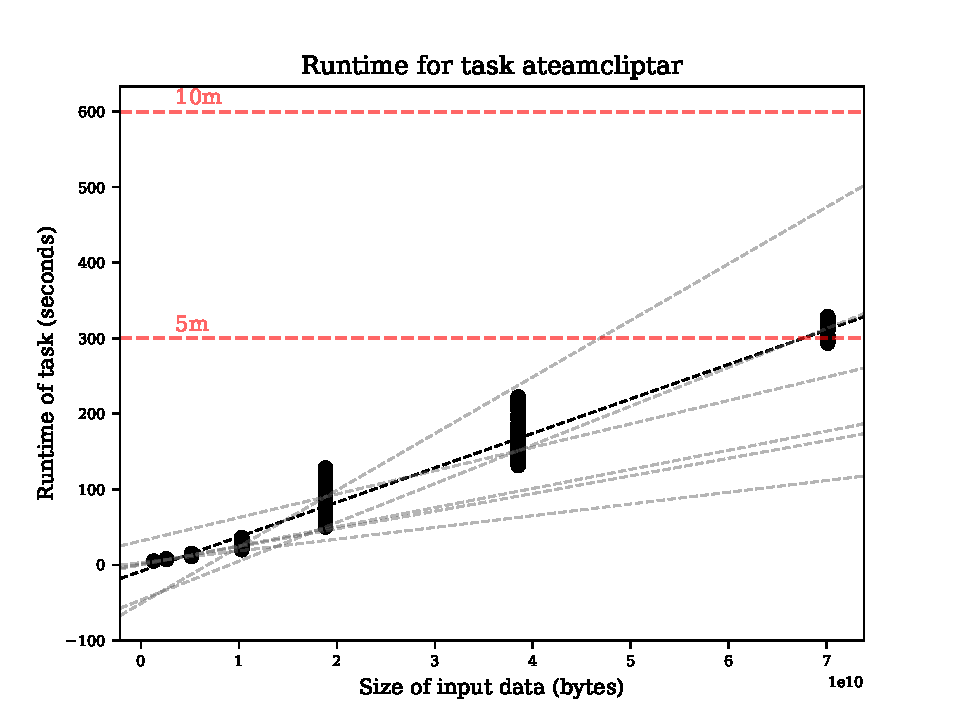
\includegraphics[width=0.95\linewidth]{figures/ateamcliptar_size.pdf}
      \caption{Tests of the ateamcliptar step for input data size ranging from 1GB to 64 GB. This step removes the contamination from bright off-axis sources. We can see that the data fits a linear model. We show the model in Equation \ref{eq:ateamcliptar} in black.}
	\label{fig:ateamcliptar}
\end{figure}

\begin{figure}
    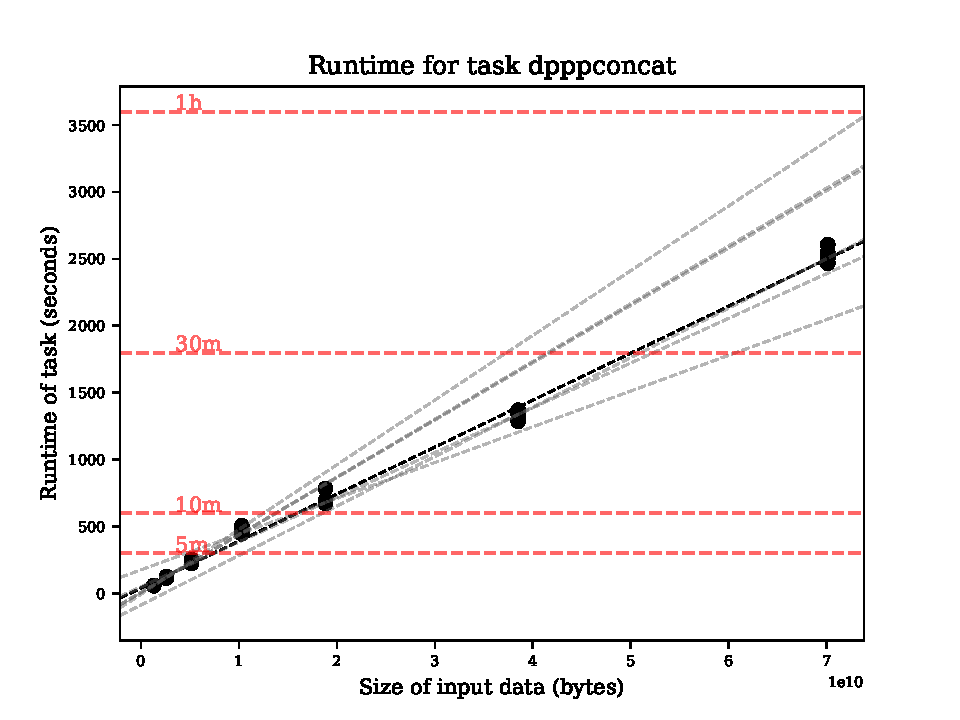
\includegraphics[width=0.95\linewidth]{figures/dpppconcat_size.pdf}
      \caption{Tests of the dpppconcat step for input data size ranging from 1GB to 64 GB. This step concatenates 10 files into a single measurement set.  We can see that the data fits a linear model. We show the model in Equation \ref{eq:dpppconcat}  in black.}
	\label{fig:dpppconcat_size}
\end{figure}

\begin{figure}
    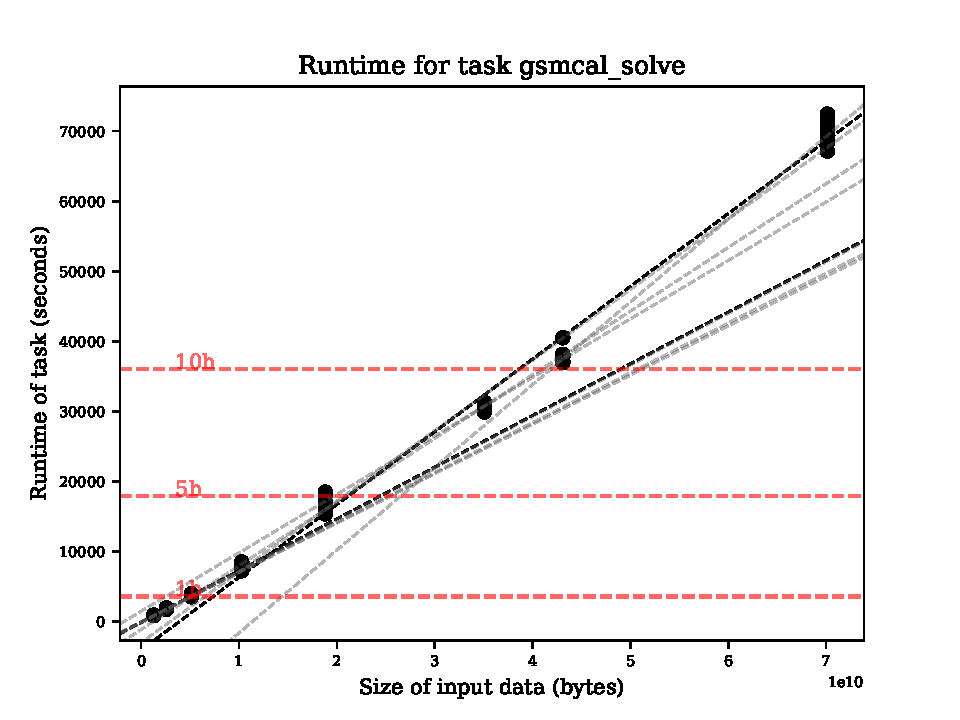
\includegraphics[width=0.95\linewidth]{figures/gsmcal_solve_size2.pdf}
      \caption{Tests of the gsmcal\_solve step for input data size ranging from 1GB to 64 GB. This step performs gain calibration of the concatenated data set against a sky model. It is the slowest and most computationally expensive \texttt{prefactor} step. We fit two linear models, for data below 16GB and above 16GB. We can see the two models, shown in  (Equation \ref{eq:gsmcalsolve}) as two black dashed lines, intersecting at 1GB.}
	\label{fig:gsmcalsolve_size}
\end{figure}

\begin{figure}
    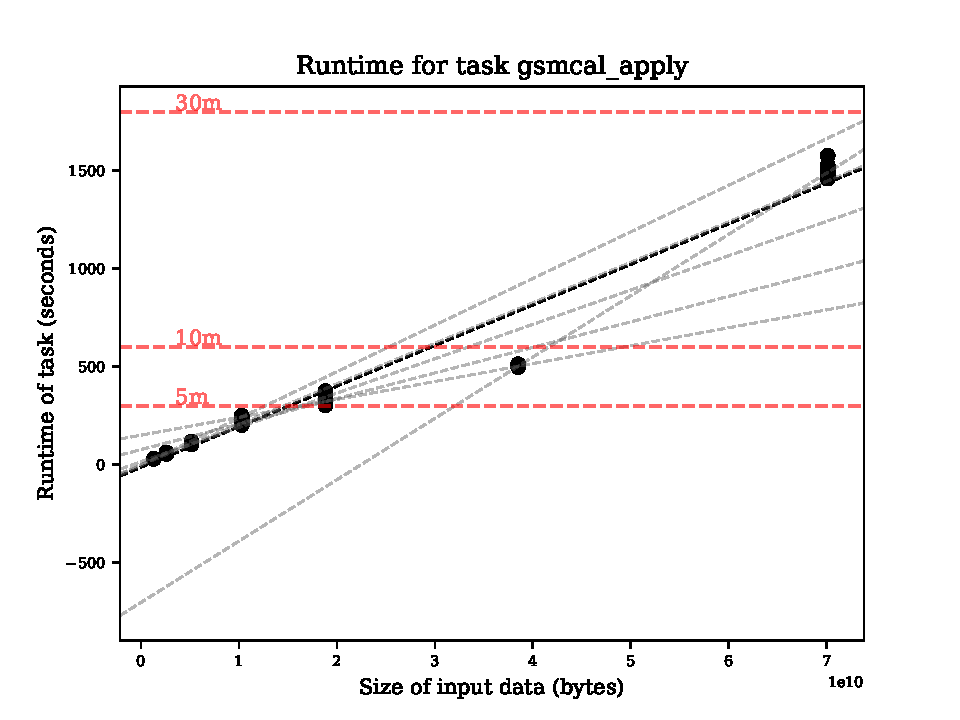
\includegraphics[width=0.95\linewidth]{figures/gsmcal_apply_size.pdf}
      \caption{Tests of the gsmcal\_apply step for input data size ranging from 1GB to 64 GB. This step applies the calibration solutions to the data. We can see that the data fits a linear model, desribed in Equation\ref{eq:gsmcalapply}, in the black dashed line.}
	\label{fig:gsmcalapply_size}
\end{figure}

\subsubsection{Calibration Model Size}
To test the effect of the calibration model size on run time, we tested our calibration with several different lengths of the sky model file. We created these models by changing the minimum sensitivity using values ranging from 0.05 Jy to 1.5 Jy. The most sensitive model (0.05 Jy) had 809 sources while the 1.5 Jy model had only 16 sources. 

Figure \ref{fig:skymodel_run_lenght} shows that the calibration time is directly proportional to the length of the sky model. Figure \ref{fig:skymodel_run_sens} shows the run time as a function of the processing parameter: the cutoff sensitivity. As the relationship between the number of sources and cutoff sensitivity is a power law, here we see the same relationship holding for processing time.

We model the run time as a function of the cutoff frequency using a power law, and fit the data to the function $y=\alpha\cdot \mathcal{F}^{-k}$. Our fit found the best model to be shown in Equation \ref{eq:skymodel_flux}, where $\mathcal{F}$ value is the cutoff flux in Jansky and $T$ is the run time in seconds. 

We show four images made from data sets calibrated with a 0.05Jy (top left), 0.3Jy (top right), 0.8 Jy (bottom left) and 1.5 Jy (bottom right) cutoff in Figure \ref{fig:skymodel_images}. The statistics for the four images, taken from the regions in green on Figure \ref{fig:skymodel_images}) are shown in Table \ref{table:skymodel_RMS}. We discuss the implication and caveats of these results in Section \ref{sec:discussions}.


\begin{table}[h!]
\centering
\begin{tabular}{||p{3cm}| c | c ||} 
 \hline
 Calibration Model Flux Cutoff & \# of sources& RMS Noise (Jy) \\  \hline
 0.05Jy & 809 &0.00402834   \\   \rowcolor{Gray}
  \hline
 0.3 Jy & 180 &0.00402311 \\  \hline
 0.8 Jy & 49 &0.00404181 \\  1.5 Jy & 16 &0.00410204 \\  \hline
\end{tabular}
\caption{Statistics for an empty region for the four images shown in Figure \ref{fig:skymodel_images}. The 0.3Jy model, here shown shaded in gray,  is the one used in production.  }
\label{table:skymodel_RMS}
\end{table}

\begin{equ}
\begin{equation}
    T=1185\cdot \mathcal{F}^{-0.854}
\label{eq:skymodel_flux}
\end{equation}
\caption{Processing time for the gsmcal\_solve step as a function of the flux cutoff of the calibration model ($\mathcal{F}$) in Jansky}
\end{equ}

\begin{figure}
    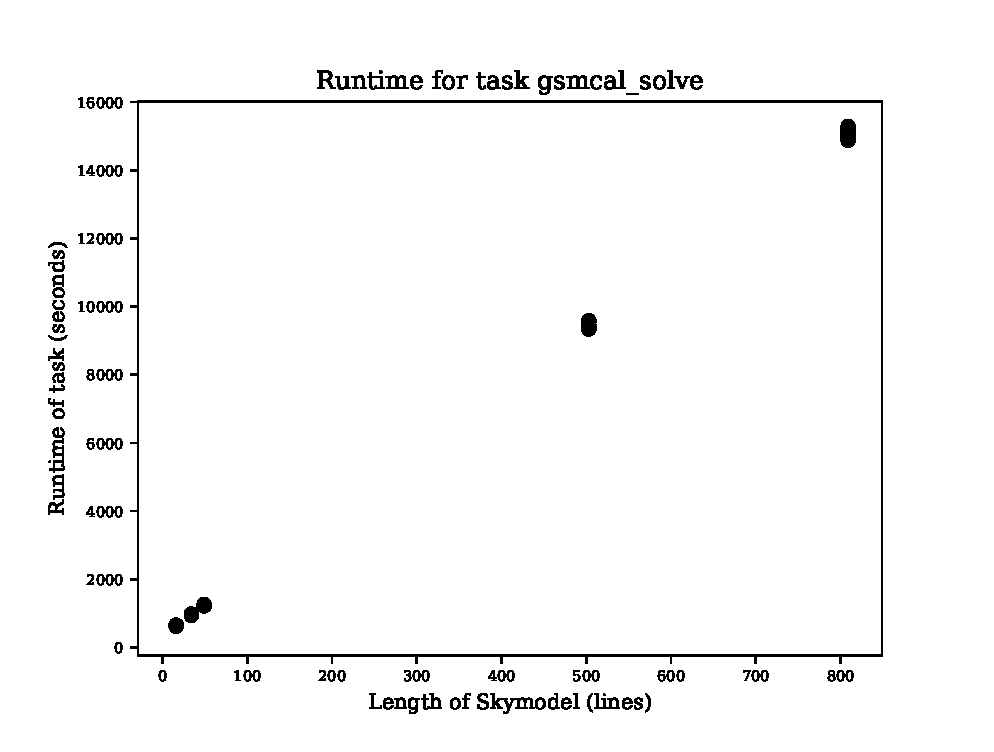
\includegraphics[width=0.95\linewidth]{figures/skymodel_length.eps}
      \caption{The processing time of the gsmcal\_solve step is linear with the size of the sky model as measured by the number of sources.}
	\label{fig:skymodel_run_lenght}
\end{figure}

\begin{figure}
    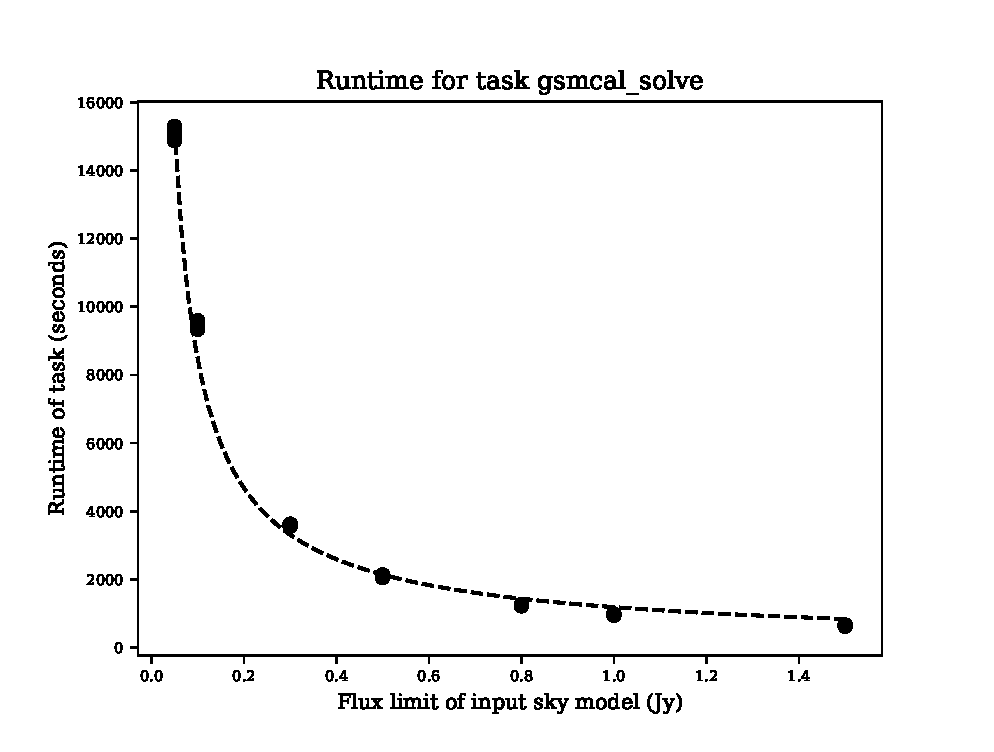
\includegraphics[width=0.95\linewidth]{figures/skymodel_flux.eps}
      \caption{The run time of the gsmcal\_solve step as a function of the cutoff sensitivity is not linear. As shown in Figure \ref{fig:skymodel_size}, the number of sources increases exponentially as the minimum sensitivity decreases. The dashed line shows the model fitted in Equation \ref{eq:skymodel_flux}. }
	\label{fig:skymodel_run_sens}
\end{figure}

\begin{figure*}
    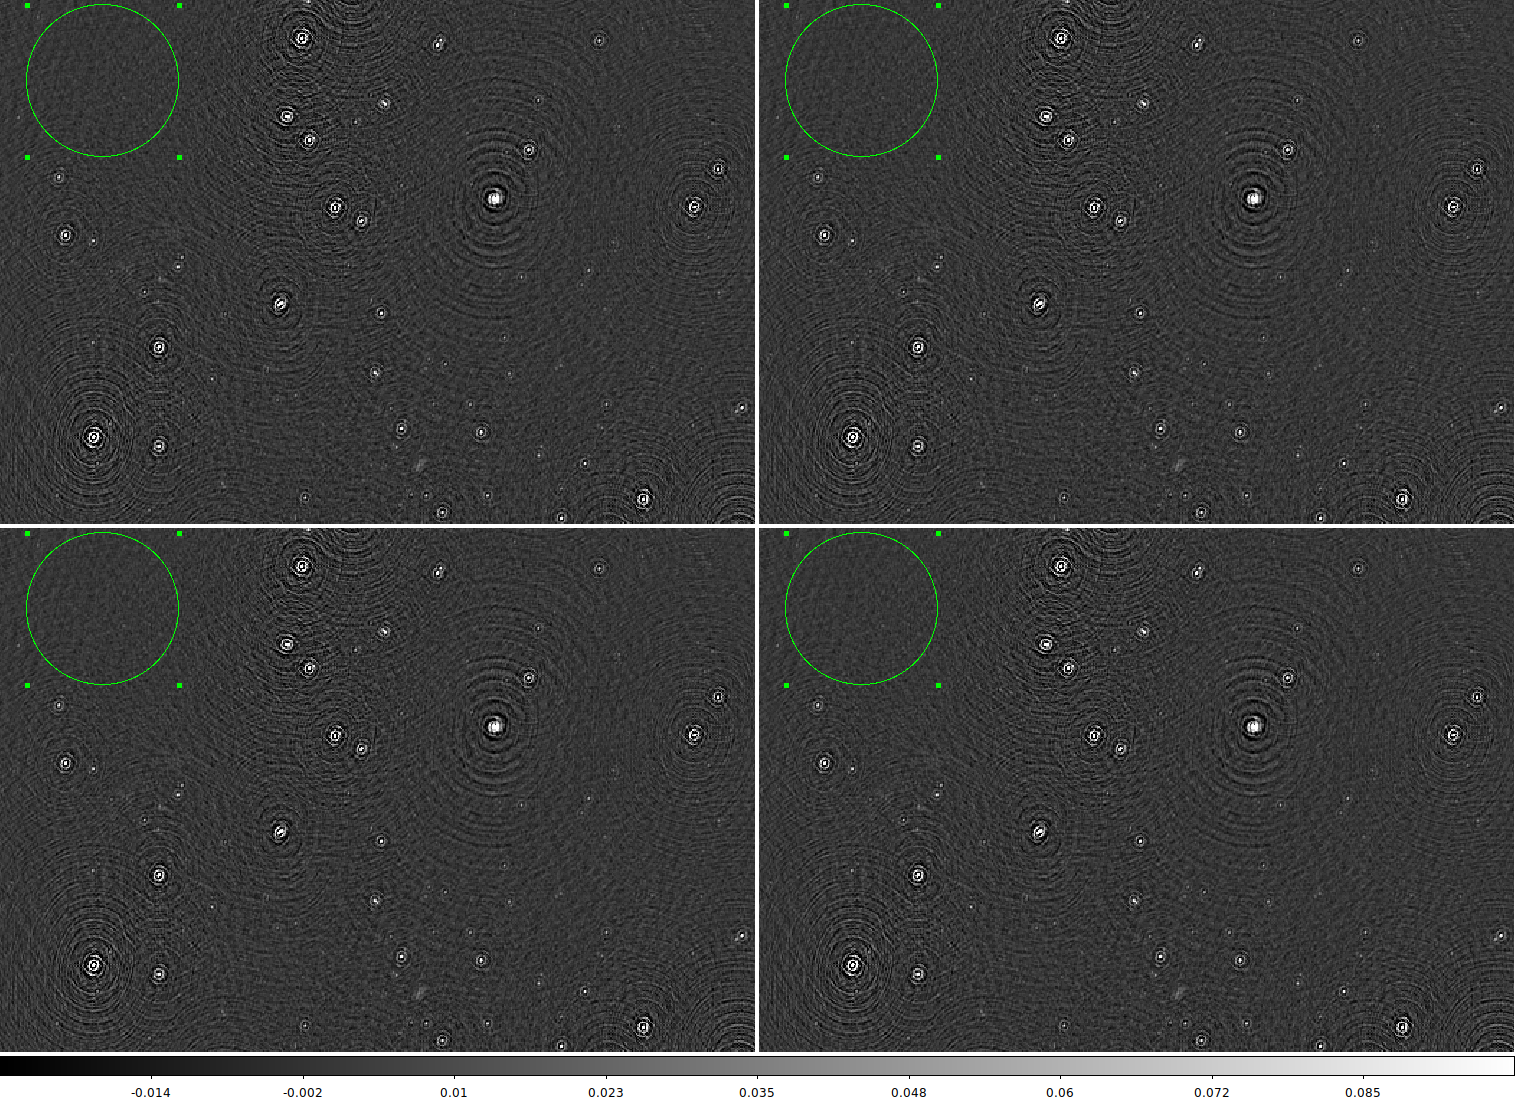
\includegraphics[width=0.95\linewidth]{figures/skymodel_images.png}
      \caption{Four images made using the \texttt{wsclean} software \citep{wsclean} from the data set\protect\footnotemark. The four images were calibrated with sky models of various flux cutoffs ranging from 0.05Jy (top left) to 1.5Jy (bottom right). Flux statistics for the green regions in the four images are listed in Table \ref{table:skymodel_RMS}. We can see that the images do not differ significantly in quality, artefacts, and noise levels. While the images have similar noise statistics, the data for the top left image takes $\sim$10 times longer to calibrate than that for the bottom right image. }
	\label{fig:skymodel_images}
\end{figure*}
\footnotetext{Using the command wsclean -absmem 50 -niter 3 -size 4096 4096 -scale 20asec}
\subsubsection{Number of CPUs}
One further parameter that can be optimized is the number of CPUs requested when the job is launched. We investigated the processing speedup as a function of the number of CPUs for the \texttt{prefactor} target pipeline. From the steps tested, only the gsmcal\_solve step shows a significant speedup as the number of CPUs is increased. The run time of this step is an inverse power law with respect to the number of CPUs as seen in Figure \ref{fig:gsmcal_solve_NCPU}. Unlike the solving step, the step applying the calibration solutions (gsmcal\_apply) is constant in time with respect to the number of CPUs as seen in Figure \ref{fig:gsmcal_apply_NCPU}. 

We fit a model with processing time inversely proportional to the number of CPUs used. We show the resulting model in Equation \ref{eq:gsmcal_NCPU}, with the parameter $(\mathcal{N})$ being the number of CPUs used. 

\begin{figure}
    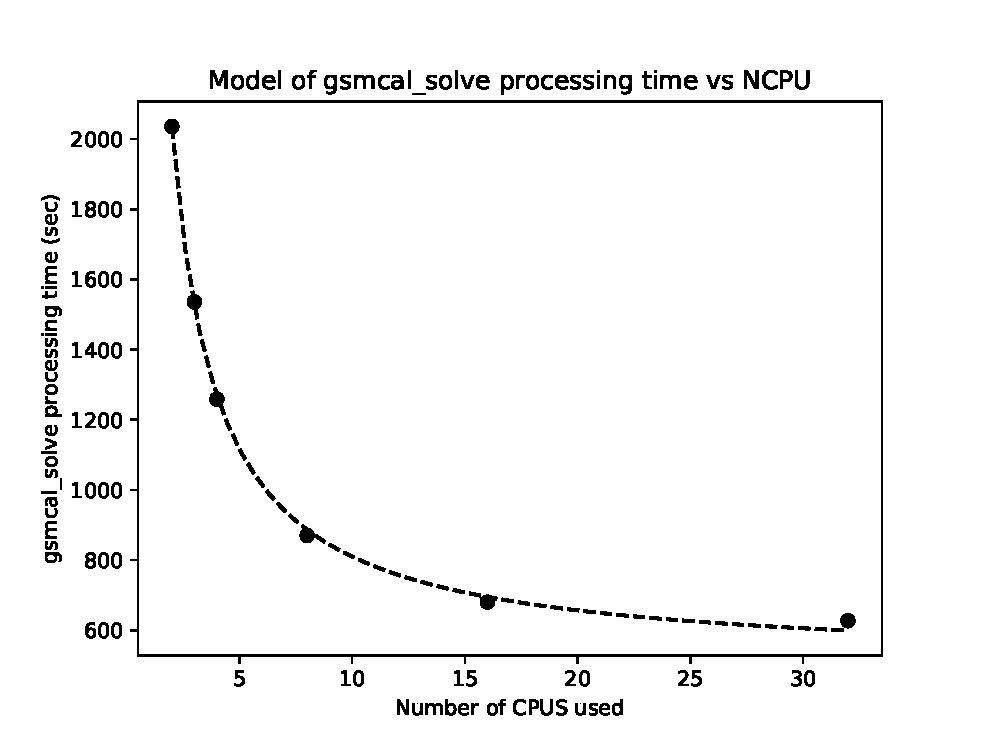
\includegraphics[width=0.95\linewidth]{figures/gsmcal_NCPU_and_model.eps}
      \caption{The processing time of the gsmcal\_solve step decreases exponentially with the number of CPUs requested. The model in Equation \ref{eq:gsmcal_NCPU} is shown in a dashed line. As this is a 1/x model, it shows diminishing returns past 16 CPUs. }
	\label{fig:gsmcal_solve_NCPU}
\end{figure}

\begin{figure}
    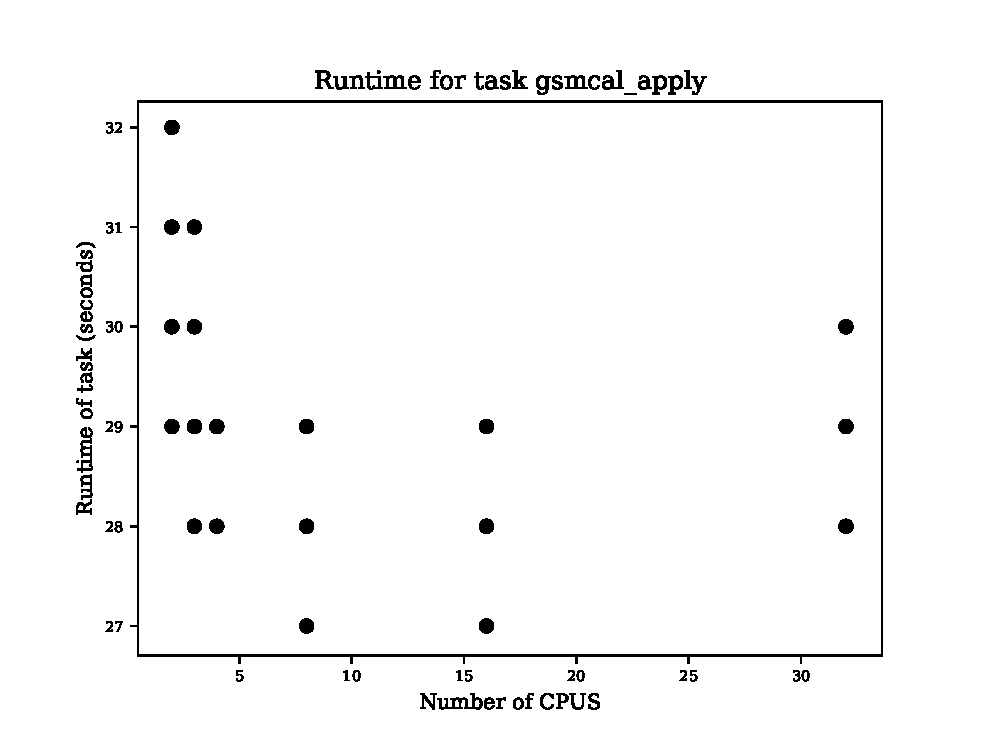
\includegraphics[width=0.95\linewidth]{figures/gsmcal_apply_NCPU.eps}
      \caption{The step that applies the calibration solutions, gsmcal\_apply, does not show a speedup when run on multiple cores, as all runs take roughly 30 seconds to complete.  }
	\label{fig:gsmcal_apply_NCPU}
\end{figure}

\begin{equ}
\begin{equation}
    T=503.37+\frac{3062.6}{\mathcal{N}}
\label{eq:gsmcal_NCPU}
\end{equation}
\caption{Processing time for the gsmcal\_solve step as a function of ($\mathcal{N}$), the Number of CPUs used by the process.}
\end{equ}


\subsection{Queuing Tests}

Aside from performance of the LOFAR software, we measured the queuing time at the \texttt{GINA} cluster, as a function of the number of CPUs requested. This data was obtained between 16 Nov 2018 and 10 Dec 2018 for 1,  2, 3 ,4, 8, and 16 CPUs per job. A histogram of the queuing time for these jobs is shown in Figure \ref{fig:queue_NCPU}. Statistics for these runs are in Table \ref{table:queueing_stats}. We use the 75th percentile of the queuing time for each parameter step to fit a model. This scenario will include 75\% of runs and is a good trade-off between ignoring and including outliers. 

We fit two linear models for this queueing time. One model for 1-4 CPUs and one for 4-16 CPUs. The model, as a function of Number of CPUs, $\mathcal{N}$ is in equation \ref{eq:queue_model}. The two models are plotted against the 75th percentile of the queuing times (last column in Table \ref{table:queueing_stats}) in Figure \ref{fig:queue_model}.

\begin{figure}
    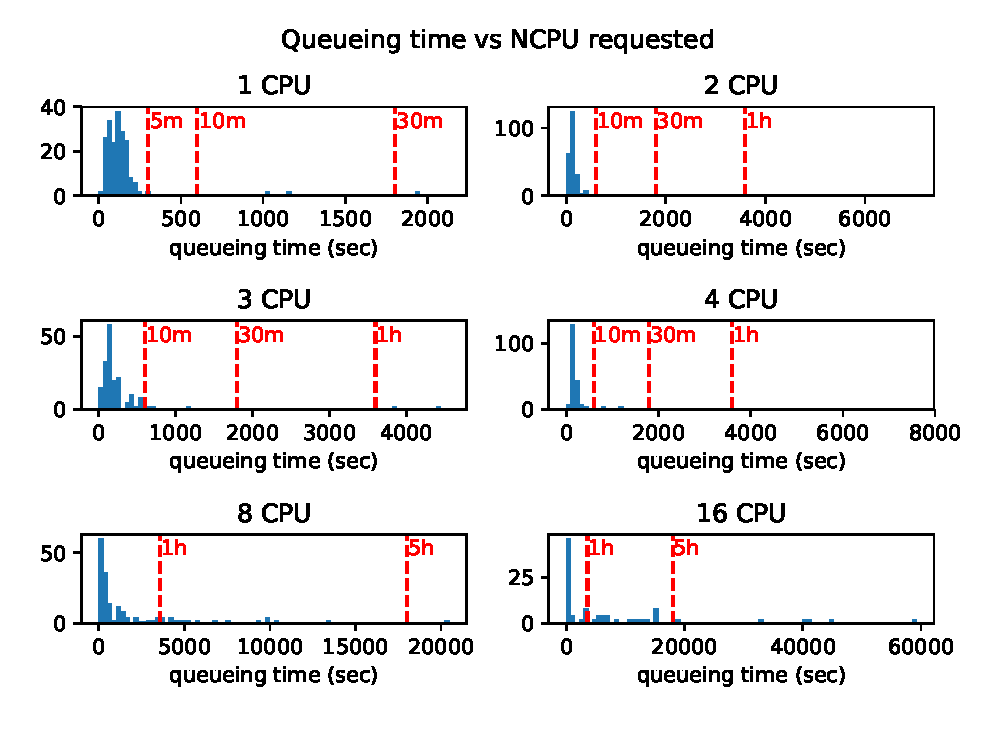
\includegraphics[width=0.95\linewidth]{figures/Queue_NCPU.eps}
      \caption{Test randomly submitting jobs to the \texttt{GINA} with different number of requested CPUs. The long tail for 8 and 16 CPU jobs shows that some jobs can take several hours to launch.  }
      
	\label{fig:queue_NCPU}
\end{figure}


\begin{table*}[t]
\centering
\begin{tabular}{||p{2.8cm}|c | c | c||} 
 \hline
 NCPU requested & Mean time (sec) & Median time (sec) & 75th percentile (sec)\\ [0.5ex]
 \hline
 1 CPU & 150.5   & 116.2 & 154.1   \\ 
 2 CPU & 201.1 & 125.8 & 165.8 \\
 3 CPU & 296.2 & 152.0 & 243.0 \\
 4 CPU & 498.9 & 167.7 & 233.7\\
 8 CPU & 1944.2 & 428.4 & 2142.4\\
 16 CPU & 7079.0 & 696.4 & 8750.6\\
 \hline
\end{tabular}
\caption{Statistics for queuing time for different values of CPUs requested. Queueing time for jobs requesting less than 8 CPUs is typically less than five minutes. It can drastically increase for larger jobs. }
\label{table:queueing_stats}
\end{table*}

\begin{figure}
    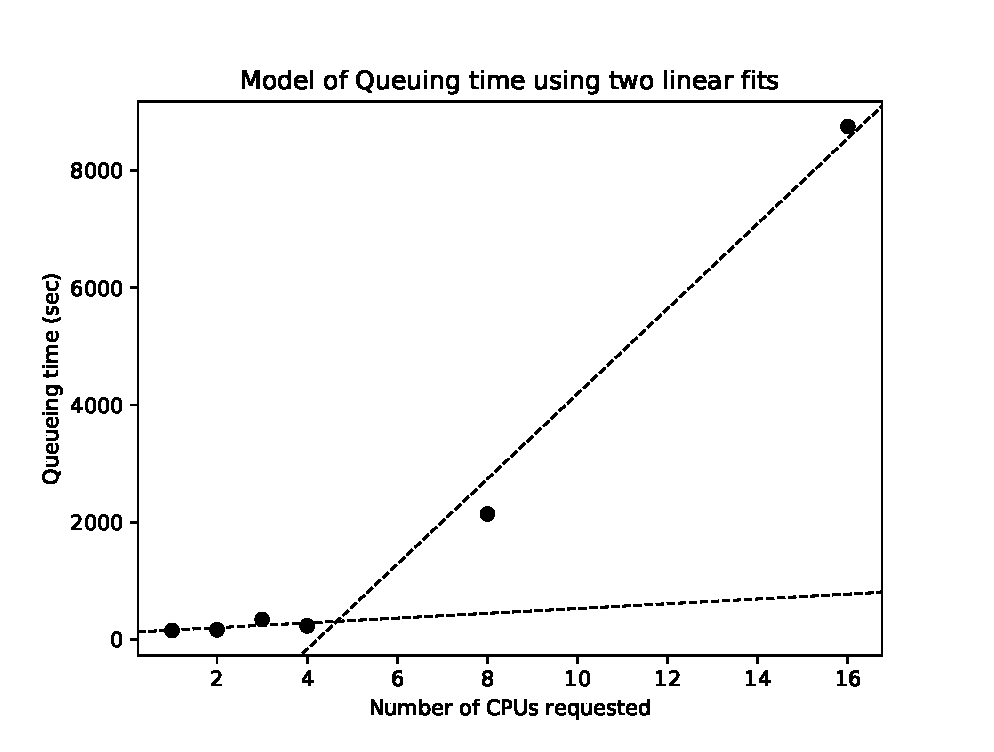
\includegraphics[width=0.95\linewidth]{figures/Queueing_model.eps}
      \caption{The queuing model built from two linear fits to the queuing times. We use the 75th percentile of the queuing data as a upper bound of job queuing. }
	\label{fig:queue_model}
\end{figure}

\begin{equ}
\begin{equation}
  T = \begin{cases}
    49.3\cdot\mathcal{N}+ 120 &|\mathcal{N}<=4\\
    726\cdot\mathcal{N}-3071 & |\mathcal{N}>4
    \end{cases}
  \label{eq:queue_model}
\end{equation}
\caption{The model for the Queuing time as described by two linear models. }
\end{equ}



\subsection{Transfer and Unpacking Time}\label{sec:results_dl}

We tested the downloading and unpacking time for data sizes ranging from 512MB to 64GB. We discovered that the unpacking of files below 64GB scaled linearly with file size, however unpacking individual data sets larger than 16GB becomes considerably slower than downloading it. 

Figure \ref{fig:dl_hist} shows the histogram of the download tests, and Figure \ref{fig:dl_plot} displays the tests as a function of data size. Both figures show that extracting of the 32 and 64GB data sets has more slow outliers than the downloading of this data. 

We fit a power law model to the time taken to transfer and unpack the data. In this case, we also consider the 75th percentile of these times in order to capture the majority of runs and ignore outliers. The plot of the data and our model can be seen in Figure \ref{fig:dl_plot} and the model is in Equation \ref{eq:download_model}, as a function of the input data size, $\mathcal{S} $ in Gigabytes.

\begin{figure}
    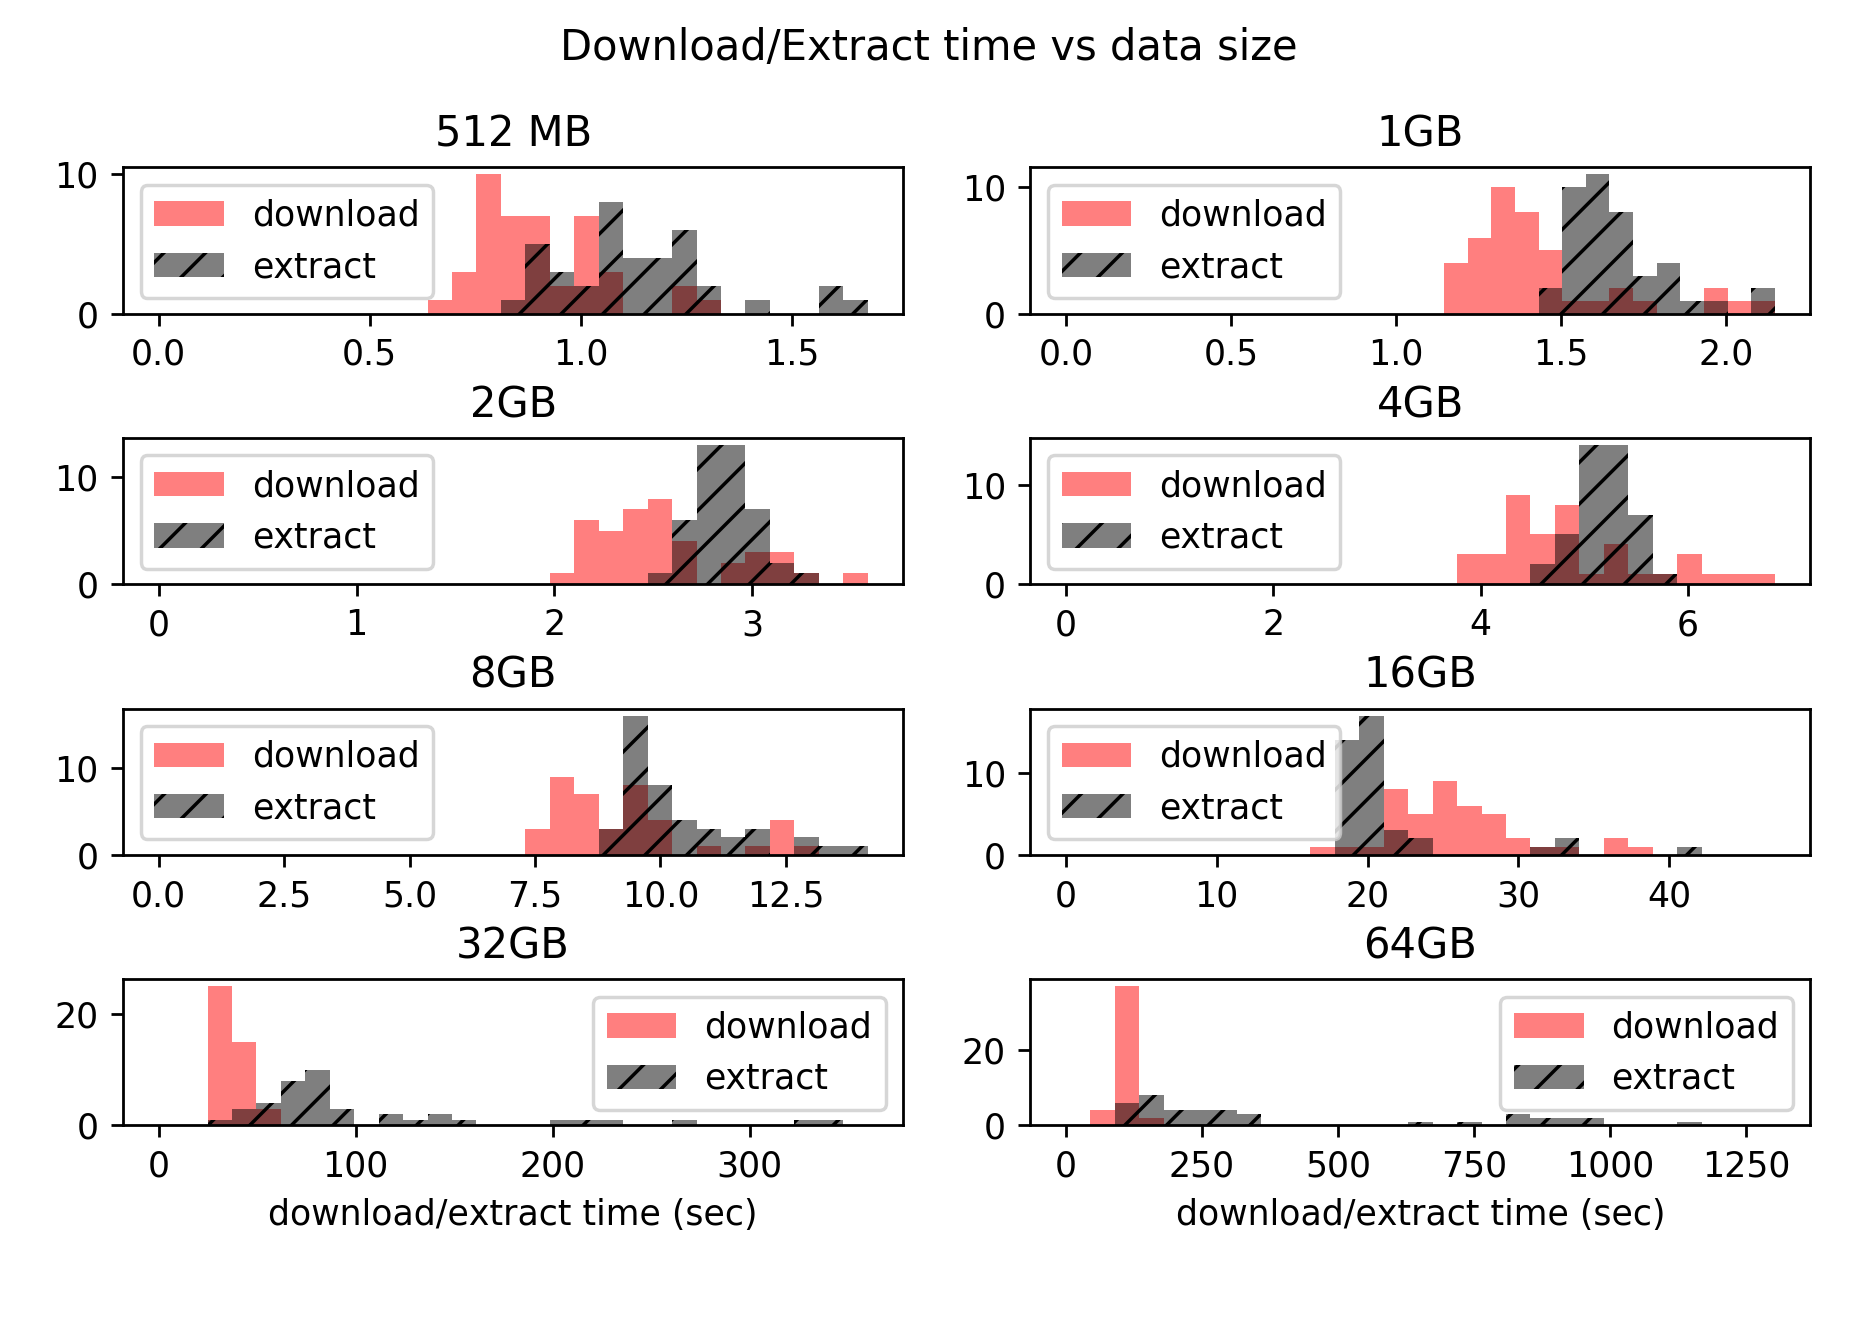
\includegraphics[width=0.95\linewidth]{figures/dl_ex_hatched.png}
      \caption{A histogram of the download and extracting times of multiple data sizes on the \texttt{GINA} worker nodes. Download and extract times are comparable for data up to 8GB, however above that, the extracting time dominates.  }
	\label{fig:dl_hist}
\end{figure}

\begin{figure}
    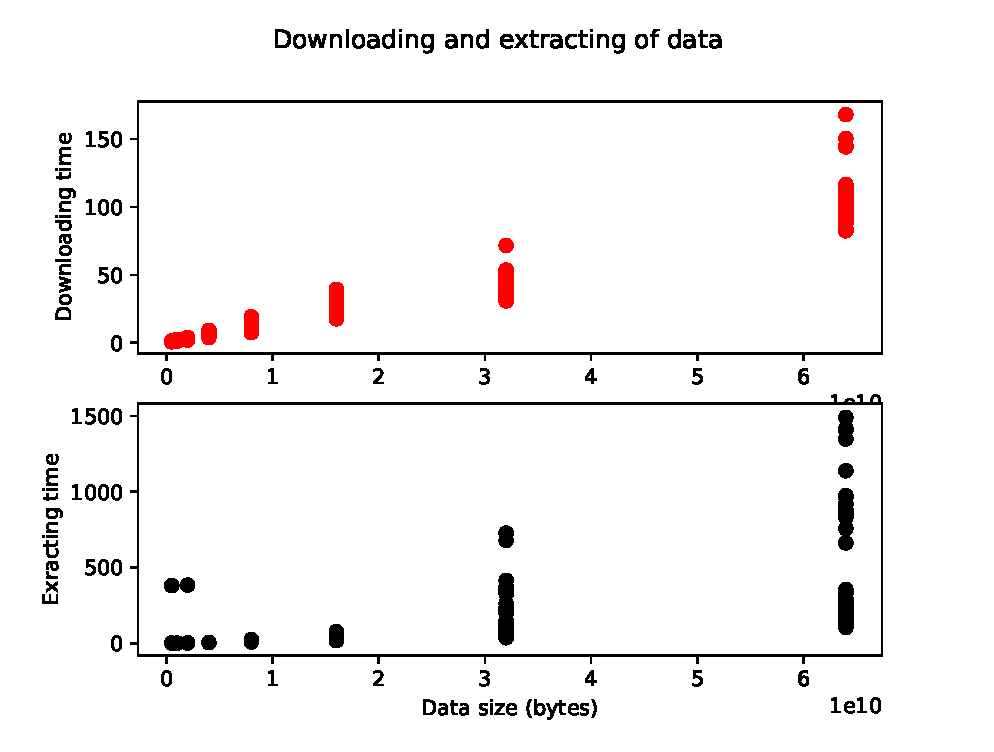
\includegraphics[width=0.95\linewidth]{figures/download_extract_sct.eps}
      \caption{A scatter plot of the download and extracting times of multiple data sizes on the \texttt{GINA} worker nodes. The difference between download and extract time for the 32 and 64 GB data sets can be seen.  }
	\label{fig:dl_plot}
\end{figure}

\begin{figure}
    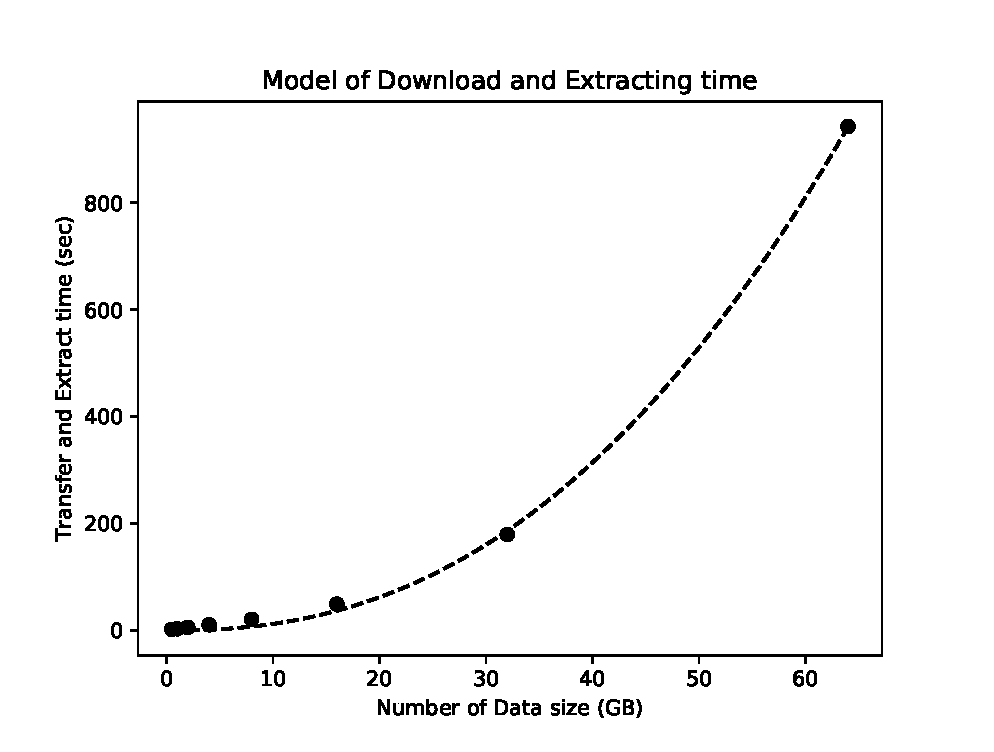
\includegraphics[width=0.95\linewidth]{figures/Dl_Ex_model.eps}
      \caption{Fit of an exponential model to the Download and Extraction time for different data sizes. For the transfer overhead, we took the 75th percentile from the data shown in Figure \ref{fig:dl_hist}. The model in Equation \ref{eq:download_model} is shown in a dahsed line. }
	\label{fig:dl_ex_model}
\end{figure}

\begin{equ}
\begin{equation}
  T=5.918\times10^{20}\cdot \mathcal{S}^{2.336}
  \label{eq:download_model}
\end{equation}
\caption{Model of the downloading and extracting time as a function of the data size ($\mathcal{S}$) in bytes.}
\end{equ}


\subsection{Comparison with production runs}
Over the past two years, the LOFAR software has been running in production and collecting data on run time for each processing step. We have saved detailed logs for these runs starting in July 2018.  We can compare this to the isolated model in order to determine the overhead incurred by processing LOFAR data on shared nodes. 

Using the logs recorded by our processing launcher\footnote{GRID\_PiCaS\_Launcher, \url{https://github.com/apmechev/GRID\_picastools }}, we made plots showing the processing time for the downloading and extracting, and for the slowest steps, ndppp\_prepcal and gsmcal\_solve. 
The results are shown in Figures \ref{fig:prod_dl_10} and \ref{fig:prod_dl_64}. We include predicted extract times from Section \ref{sec:results_dl} as vertical dashed lines for both plots. 

Finally, we present Figures \ref{fig:prod_gsmcal} which shows a comparison of gsmcal\_solve run times and our model's prediction for a 1GB data set.  Figure \ref{fig:prod_gsmcal_times} plots the processing time vs data size for these production runs and includes the model from Equation \ref{eq:gsmcalsolve}. The significant overhead incurred on a shared infrastructure can be noted. 

\begin{figure}
    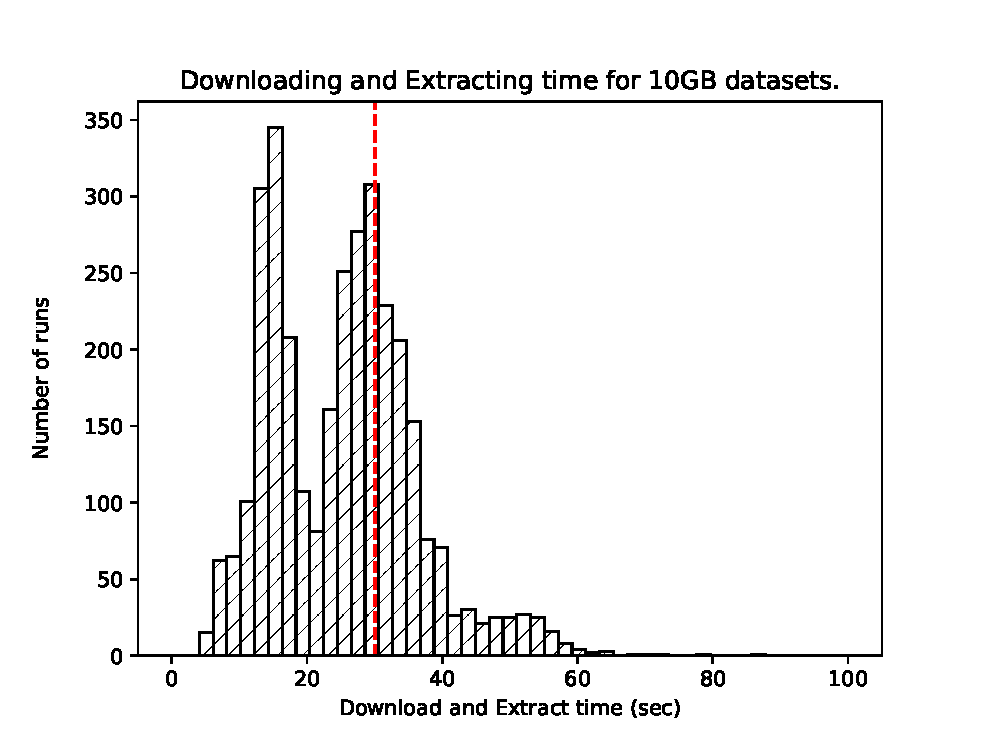
\includegraphics[width=0.95\linewidth]{figures/Production_10GB_2.eps}
      \caption{Downloading and extracting time for 10 1GB data sets performed in our production environment. Data from this test ranges from July 2018 to January 2019. The dashed red line shows the prediction obtained from section \ref{sec:results_dl}. We see a bimodal distribution corresponding to 10 GB data (right peak) and data averaged further to 5GB (left peak).}
	\label{fig:prod_dl_10}
\end{figure}


\begin{figure}
    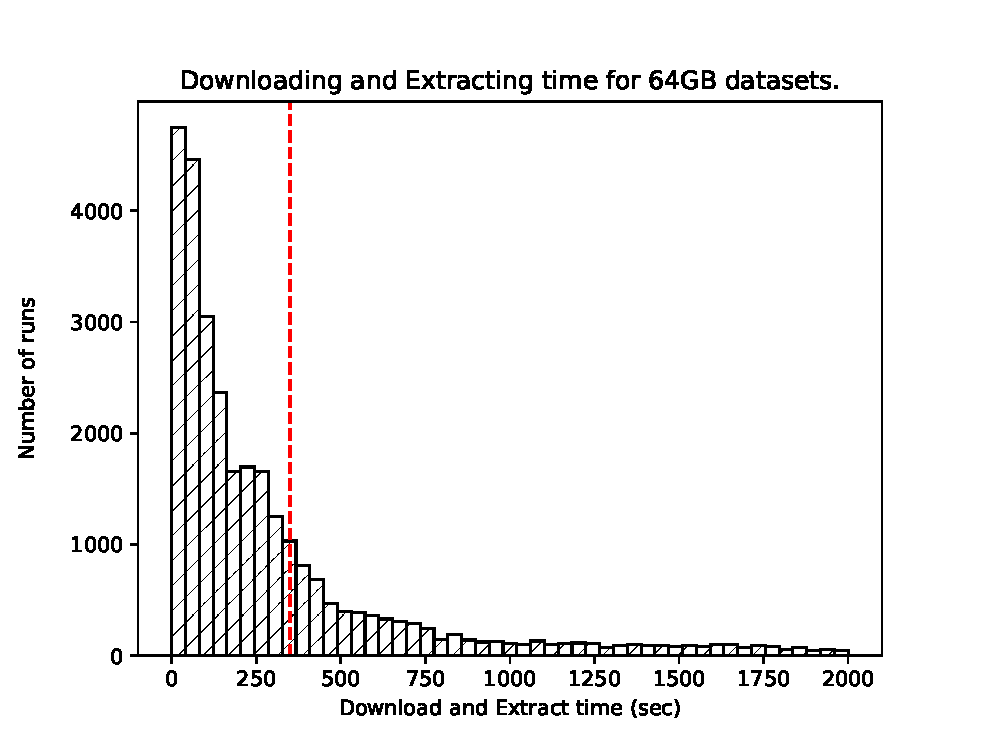
\includegraphics[width=0.95\linewidth]{figures/Production_64GB_2.eps}
      \caption{Downloading and extracting time for a 64GB data set performed in our production environment. Data from this test ranges from 07/2018-01/2019. The dashed red line shows the prediction obtained from Figure \ref{fig:gsmcalsolve_size} in Section \ref{sec:results_dl}. }
	\label{fig:prod_dl_64}
\end{figure}


\begin{figure}
    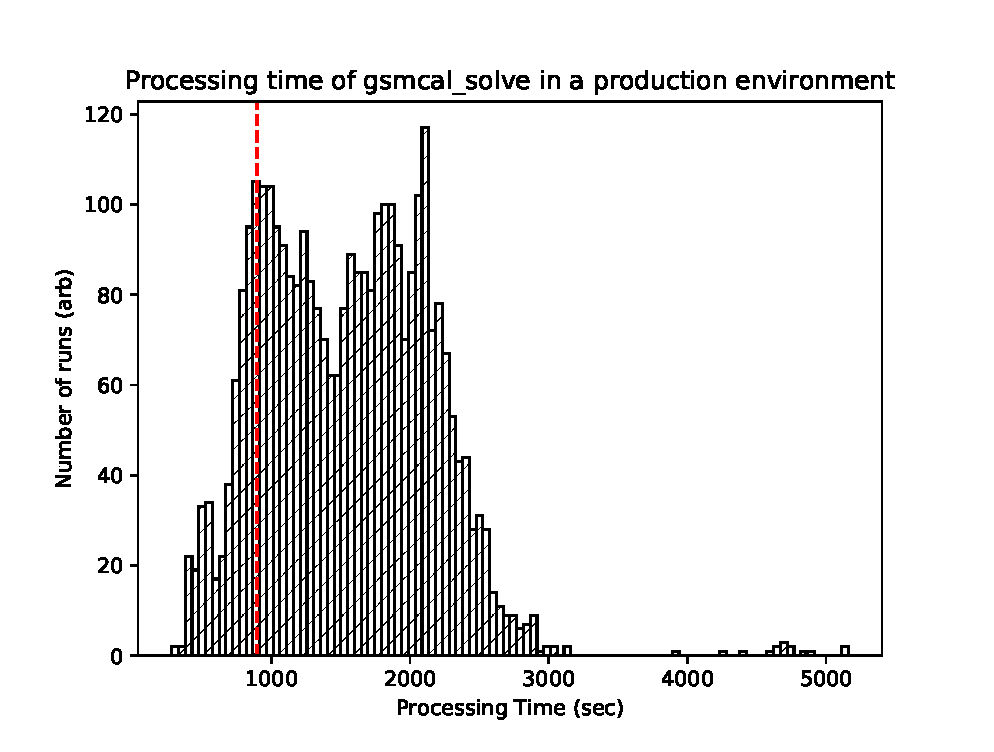
\includegraphics[width=0.95\linewidth]{figures/Production_gsmcal_1GB_2.eps}
      \caption{Processing time for the gsmcal\_solve step in a production environment. Data from this test ranges from 07/2018-01/2019. The dashed red line shows the prediction for a 1GB run, obtained from section \ref{sec:results_dl}. We see two distributions, which correspond to data averaged to 1GB and 512 MB.  It should be noted that the left peak corresponds to 512MB data, as seen in Figure \ref{fig:prod_gsmcal_times}.}
	\label{fig:prod_gsmcal}
\end{figure}


\begin{figure}
    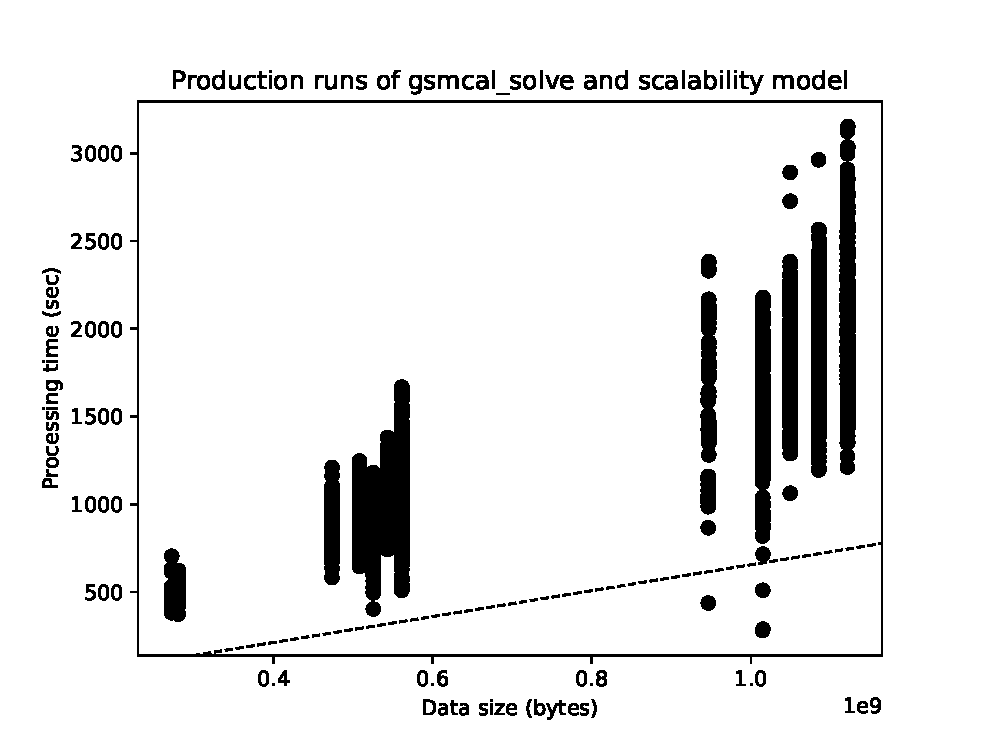
\includegraphics[width=0.95\linewidth]{figures/gsmcal_solve_size_prod.eps}
      \caption{The scalability model for processing data through the gsmcal\_solve step and the performance for production runs of this step between July 2018 and January 2019. }
	\label{fig:prod_gsmcal_times}
\end{figure}


\subsection{Complete Scalability Model}
To incorporate all our data into a complete model, we consider the slowdown of each parameter as a multiplier to the time taken to process our base run. We incorporate the models for each parameter above for the model of the run time. We add the transfer and queuing time to the processing time to obtain a final function of all our parameters. We can use this function to predict the processing time for an arbitrary data set. The final performance model is in Equation \ref{eq:full_model}. 

\begin{equ*}[!t]
\normalsize
\begin{equation}
    \begin{split}
   t_{gsmcal\_solve} & = \begin{cases}
        49.3\cdot\mathcal{N}+ 120 &|\mathcal{N}<=4\\
        726\cdot\mathcal{N}-3071 & |\mathcal{N}>4
       \end{cases} \\
       & + 0.056\cdot \mathcal{S}^{2.336} \\ 
       & + 3566\cdot \frac{1}{3.012}\mathcal{F}^{-0.854} \cdot 9.97\cdot10^{-7}\mathcal{S}\cdot (0.1412+\frac{0.8589}{\mathcal{N}}) \\
       & + 0.056\cdot \mathcal{S}^{2.336} 
       \end{split}
 \label{eq:full_model}
 \end{equation}
\caption{Model of the total time of the gsmcal\_solve step ($t_{gsmcal\_solve}$) for the parameters $\mathcal{N}$, Number of CPUs; $\mathcal{S}$, Size of data in bytes and $\mathcal{F}$, cutoff calibration model flux in Jansky. }
\end{equ*}

\section{Discussions and Conclusions}\label{sec:discussions}

The goal of this work is to understand the performance of the LOFAR Direction Independent Pipeline as processing parameters are changed. We increased the size of broadband LOFAR data by a factor of 64 in size, and discovered that all our processing steps scale linearly in time with respect of the input data size. We learned that for input data above 16GB in size, the slope of our scaling relation is higher than for the smaller data sets.

As the calibration step concatenates 10 input subbands, and the test system only has 380GB of RAM, data larger than 16GB, the discrepancy in slopes can be attributed to the large memory requirement for data larger than 200GB. Splitting the performance model in two also helps make a more accurate processing time prediction as fitting a single linear model would have a large negative y-intercept, predicting negative processing times for data smaller than 2GB. 

When comparing our model's prediction with real processing runs over the past six months, we note that there are considerable overheads when processing data on an isolated node vs when running on a shared infrastructure (Figure \ref{fig:prod_gsmcal_times}). The overhead in processing is roughly a factor of two-three from our model. This discrepancy suggests that a model for gsmcal\_solve needs to be built using data when running on a shared environment, to better predict processing time. 

Our analysis shows the following results. Overall, the slowest step was the gsmcal\_solve step, and its run time scales more strongly with data size than the other steps (equation \ref{eq:gsmcalsolve} has the steepest slope). This suggests that as data sizes increase, gsmcal\_solve will increasingly dominate the processing time over the other steps (As seen in Figures \ref{fig:predict_ateam} and \ref{fig:gsmcalsolve_size}). This effect is especially prominent for data larger than 16GB (160GB when 10 subbands are concatenated). As such, it is recommended to avoid calibration of data larger than 160GB. 

Additionally, we discovered that the calibration scales linearly in time as a function of the length of the calibration model, however it is a power law as a function of the model's cutoff sensitivity. This is because of the (expected) power law relation between the number of sources and cutoff sensitivity, seen in Figure \ref{fig:skymodel_size}. We can use this discovery to accelerate the processing time by increasing the flux cutoff to the LOFAR direction independent calibration to 0.5 Jy. Doing so will execute the calibration step in 60\% of the time, saving 83 CPU-h per run. Over the remaining 2000 \texttt{prefactor} runs left in the LOTSS project, this change in sensitivity will save more than 167k CPU hours. 

Figures \ref{fig:skymodel_images} show a data set calibrated with sky models with cutoff sensitivities listed in Table \ref{table:skymodel_RMS}, and figures  \ref{fig:skymodel_rcalib_004_03} and \ref{fig:skymodel_rcalib_08_15} show the calibration solutions obtained by calibrating with skymodels of cutoff ranging from 0.05 Jy to 1.5 Jy. These results suggest that performing gain calibration with less complex, and thus smaller, calibration models will not degrade image and solution quality while taking less than 20\% of processing time. Table \ref{table:skymodel_RMS} also confirms this result. 

While this result is encouraging, there are caveats suggesting future study is required. The results we present are for a single observation, and has not been processed through the Direction Dependent Calibration pipeline. This pipeline produces final images used for scientific research. Future work will need to confirm that a short calibration models used in the \texttt{prefactor} pipeline do not degrade the quality of these final images. 

We tested downloading and extracting test LOFAR data of various sizes. Both downloading and extracting was linear with respect to the data size for data up to 32 GB in size. Beyond those sizes, there was more scatter in data extraction due to high file-system load. This is because load on the worker node's file-system can be unpredictable and can affect the data extraction times negatively. Nevertheless, when comparing our extraction tests and processing for the past 6 months, the predictions by our models (Figure \ref{fig:dl_hist}) correspond to the production runs (Figures \ref{fig:prod_dl_10} and \ref{fig:prod_dl_64}).  
Part of the LOFAR SKSP processing is done on shared infrastructure, which requires requesting processing time ahead of time for each grant period. Being able to predict the amount of resources required to process data each grant period is required to make a reliable estimate on what resources to request. 

Moreover, providing LOFAR processing as a service to scientific users requires estimating the processing time for each request. This needs to be done in order to determine whether the user has sufficient resources left in their resource pool. Knowing the performance of the software pipelines as a function of the input parameters will help predict the run time for each request and the resources consumed. Knowing this will make it possible to notify users how long the request will take and how much of their quota will be used up. 

Finally, a performance model of the LOFAR software will help make predictions on the time and resources needed to process data for other telescopes such as the Square Kilometer Array (SKA). Once operational, the SKA is expected to produce Exabytes of data per year. Processing this data efficiently requires understanding the scalability of the software performance to facilitate scheduling and resource allotment. Overall, these results will help guide algorithm development in radio astronomy, as well as be useful to schedule future processing jobs and optimize resource usage. 


\appendix

\renewcommand{\theequ}{\Alph{section}.\arabic{equ}}


\section{Calibration Solutions for the sky model tests }\label{ap:calib_solutions}
The output of the calibration step is a data set corrected for direction independent effects, as well as a set of calibration solutions. Figures \ref{fig:skymodel_rcalib_004_03} and \ref{fig:skymodel_rcalib_08_15} show the calibration solutions for core station obtained when calibrating with  sky models with minimum flux cutoffs of 0.05, 0.3, 0.8 and 1.5Jy. Much like in Figure \ref{fig:skymodel_images}, we can see that there is no significant difference between the calibration solutions for these stations. 

\begin{figure}
    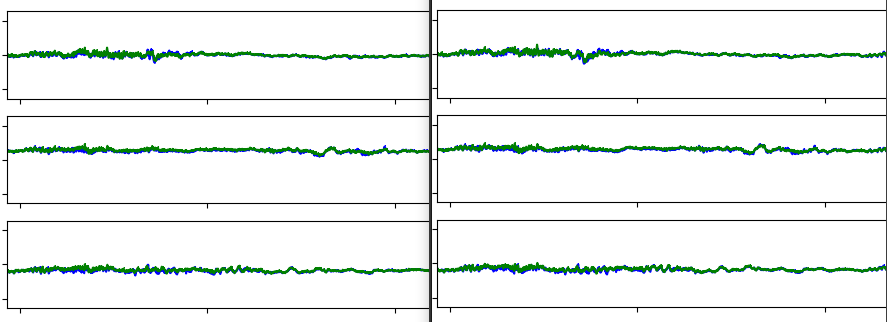
\includegraphics[width=0.95\linewidth]{figures/005_and_03_solutsions_CS003HBA0_CS003HBA1_CS004HBA0.png}
      \caption{The calibration (phase) solutions for the test dataset obtained when calibrating with sky models of 0.05 Jy cutoff (left) and 0.3Jy cutoff (right). The data shows the phase solutions for baselines including stations CS003HBA0, CS003HBA1 and CS004HBA0, with respect to the reference station, CS001HBA0. The right solutions were obtained using the production calibration model. We do not see any improvement in results in the left figure, which took twice as long to obtain.}
	\label{fig:skymodel_rcalib_004_03}
\end{figure}


\begin{figure}
    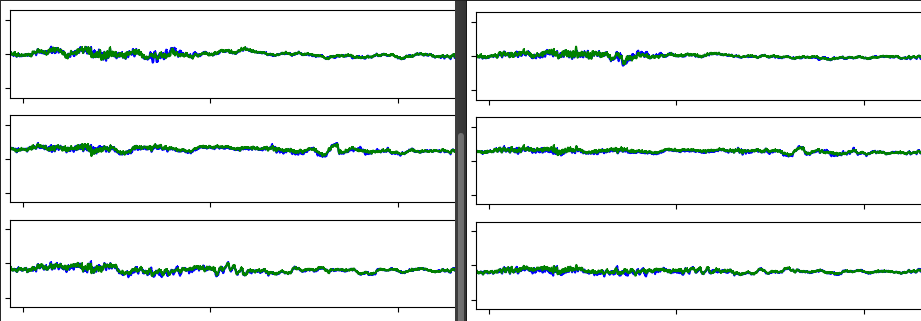
\includegraphics[width=0.95\linewidth]{figures/08_and_15_solutsions_CS003HBA0_CS003HBA1_CS004HBA0.png}
      \caption{The calibration (phase) solutions for the test dataset obtained when calibrating with sky models of 0.8 Jy cutoff (left) and 1.5Jy cutoff (right). The data shows the phase solutions for baselines including stations CS003HBA0, CS003HBA1 and CS004HBA0, with respect to the reference station, CS001HBA0. We can see that the calibration solutions shown here are not significantly different than those shown in \ref{fig:skymodel_rcalib_004_03}, despite taking a fraction of the processing time.  }
	\label{fig:skymodel_rcalib_08_15}
\end{figure}

\section{Parametric model parameters and fit accuracy}\label{ap:model_params}

In this section, we note the uncertainties to the models fit in Equations \ref{eq:runtime_size_models}-\ref{eq:download_model}. 

\numberwithin{equation}{section}
\setcounter{equation}{6}
\renewcommand{\theequation}{\Alph{section}.\arabic{equation}}

\subsection{Fits quality of run time vs input size model}

The models of the processing time vs input size were fit as a linear regression. In this work we present such models for the gsmcal\_solve, gsmcal\_apply, dpppconcat, predict\_ateam and ateamcliptar, the five slowest steps. The resulting models, calculated by the \texttt{scipy linregress}\citep{scipy} routine, are shown in Equation \ref{eq:runtime_size_models}. We present the $R^2$ values, P values and standard error below, in Table \ref{table:fits_size}.



\begin{table}[ht!]
\centering
\begin{tabular}{||p{2.2cm}| c | c|p{2cm}||} 
 \hline
 \texttt{prefactor} step & $R^2$ & P value & Standard Error \\ [0.5ex]
 \hline
 predict\_ateam & 0.996   & 0                    & $1.92\times10^{-10}$    \\ 
 \hline
 ateamcliptar   & 0.979   & 0                    & $3.94\times10^{-11}$    \\ 
 \hline
 dpppconcat     & 0.999   & $1.2\times10^{-128}$ & $1.78\times10^{-10}$    \\ 
 \hline
 gsmcal\_solve $<=$16GB  & 0.995   & $3.12\times10^{-75}$ & $6.80\times10^{-9}$     \\ 
 \hline
 gsmcal\_solve $>$16GB  & 0.951   & $7.07\times10^{-40}$ & $1.58\times10^{-8}$     \\ 
 \hline
 gsmcal\_apply  & 0.989   & $5.6\times10^{-82}$  & $3.12\times10^{-10}$    \\ 

\hline
\end{tabular}
\caption{Fit parameters for the models in Equation \ref{eq:runtime_size_models}. }
\label{table:fits_size}
\end{table}


\subsection{Fit of run time vs calibration model flux cutoff }

The run time vs Flux cutoff model shown in Equation \ref{eq:skymodel_flux} is defined by the equation $y=a\cdot x^{-k}$ and two parameters, $a$ and $k$. The covariance matrix for these two parameters is shown in Equation \ref{eq:cov_Flux}. The standard deviation for the fit of the parameters $a$ and $k$ is 26.134 and $7.624\times10^{-3}$ respectively.

\begin{equ}
\begin{equation}
  \begin{bmatrix}
    6.83\times10^{2}  &  -1.94\times10^{-1} \\
   -1.94\times10^{-1} &   5.81\times10^{-5} \\
\end{bmatrix}
\end{equation}
\caption{The covariance matrix of the parameters in model in Equation \ref{eq:skymodel_flux}.}
\label{eq:cov_Flux}
\end{equ}

\subsection{Fit of the NCPU model }
The covariance matrix for the fit parameters of equation \ref{eq:gsmcal_NCPU}, $a$ and $k$ in $y=a+\frac{k}{\mathcal{N}}$ are shown in Equation \ref{eq:cov_NCPU}. The standard deviation of the fits for $a$ and $k$ are 13.11 and 48.20 respectively. 

\begin{equ}
\begin{equation}
  \begin{bmatrix}
    171.94 & -504.11 \\
    -504.11 & 2322.95
\end{bmatrix}
\end{equation}
\caption{The covariance matrix for the parameters for the model predicting run time vs Number of CPUs used, shown in Equation \ref{eq:gsmcal_NCPU}.}
\label{eq:cov_NCPU}
\end{equ}

\subsection{Fit for the queuing time model}

The statistics of the model fit parameters for the queuing time model (Equation \ref{eq:queue_model}) are in Table \ref{table:fits_queue}. 
The queuing model is fit to the $75^{th}$ percentile of the queuing times for each parameter step. Since this results in a single number for each step, the model's P values are larger than the models from the other sections. 

\begin{table}[ht!]
\centering
\begin{tabular}{||p{2.2cm}| c | c|p{2cm}||} 
 \hline
 Value of $\mathcal{N}$ & $R^2$ & P value & Standard Error \\ [0.5ex]
 \hline
 $\mathcal{N}\leq4$ & 0.382   & 0.381                   & 37.086    \\ 
 $\mathcal{N}>4$    & 0.986   & 0.075                   & 86.293    \\ 
\hline
\end{tabular}
\caption{Goodness of fit parameters for the model in Equation \ref{eq:queue_model}. Since the model is split into two parts, we treat each section as a single linear model.}
\label{table:fits_queue}
\end{table}


\subsection{Fit of the download and extract model }
Equation \ref{eq:cov_downl} shows the covariance matrix for the two parameters  $a$ and $k$, $y=a\times10^{k}$ with the best fit values shown in Equation \ref{eq:download_model}. The standard deviations of the fits for $a$ and $k$ are 0.016 and 0.068 respectively. 

\begin{equ}
\begin{equation}
  \begin{bmatrix}
    2.53\times10^{-4} & 1.08\times10^{-3} \\
    1.08\times10^{-3} & 4.60\times10^{-3}
\end{bmatrix}
\end{equation}
\caption{The covariance matrix for the parameters for the model for Download and Extract time, shown in Equation \ref{eq:download_model}.}
\label{eq:cov_downl}
\end{equ}
 
\section*{Acknowledgements}
APM would like to acknowledge the support from the NWO/DOME/IBM programme ``Big Bang Big Data: Innovating ICT as a Driver For Astronomy'', project \#628.002.001.

This work was carried out on the Dutch national e-infrastructure with the support of SURF
Cooperative through grants e-infra 160152 and e-infra 180169.

\section*{References}
\bibliography{bibliography}

\end{document}
